\documentclass[10pt]{mypackage}

% sans serif font:
%\usepackage{cmbright,sfmath,bbold}
%\renewcommand{\mathcal}{\mathtt}

%Euler:
\usepackage{newpxtext,eulerpx,eucal,eufrak}
\renewcommand*{\mathbb}[1]{\varmathbb{#1}}
\renewcommand*{\hbar}{\hslash}

%kp fonts:
%\usepackage{kpfonts}
%\renewcommand{\mathbb}{\mathds}

\usepackage{microtype}
\pagestyle{fancy} %better headers
\fancyhf{}
\rhead{Avinash Iyer}
\lhead{Partial Differential Equations: Class Notes}

\setcounter{secnumdepth}{0}

\begin{document}
\renewcommand{\arraystretch}{1.5}
\RaggedRight
\section{Introduction}%
Consider the equations
\begin{align*}
  \frac{d^2y}{dx^2} + y(x) &= e^x\tag*{(1)}\\
  \diff{^{17}y}{x^{17}}(x) + \sin\left(y(x)\right) &= \left(x^{x}\right)^{x}\tag*{(2)}
\end{align*}
Before we want to solve these equations, we need to understand what these equations \textit{are}. 
\begin{enumerate}[(1)]
  \item This is a second order, inhomogeneous, linear ordinary differential equation.
  \item This is a 17th order, inhomogeneous, nonlinear ordinary differential equation.
\end{enumerate}
Generally, when we have a nonlinear equation, we convert it (using the Jacobian) to the ``nearest'' corresponding linear equation using Taylor approximations. In this case, converting equation (2), we have
\begin{align*}
  \diff{^{17}y}{x^{1y}}(x) + y(x) &= \left(x^{x}\right)^{x}.\tag*{(2')}
\end{align*}
Now, equation (2') is linear, so it is able to be solved. It may not be pretty,\footnote{Citation needed.} but it can be solved, using Laplace Transforms or other methods.
\section{Ordinary Differential Equations}%
Returning to our equation (1), 
\begin{align*}
  \frac{d^2y}{dx^2} + y(x) &= e^x,\tag*{(1)}
\end{align*}
there is one more fact that we can see --- this is an equation with constant coefficients. The most general form of a $n$th order linear ordinary differential equation is of the form
\begin{align*}
  a_n(x)\diff{^ny}{x^n}(x) + a_{n-1}(x)\diff{^{n-1}y}{x^{n-1}}(x) + \cdots + a_1(x)\frac{dy}{dx} + a_0(x)y(x) = g(x).\label{eq:general_linear_ode}\tag{\textdagger}
\end{align*}
Specifically, we also require $a_k(x)\in C(I)$, where $I$ is some interval (specifics will be detailed later).
\begin{theorem}[Existence and Uniqueness Theorem]
  Any ordinary differential equation of the form (\textdagger) has unique solutions in the interval $I$.\newline

  There are $n$ linearly independent solutions for $g(x) = 0$.
\end{theorem}
The corresponding homogeneous equation for (1) is
\begin{align*}
  \frac{d^2y}{dx^2} + y(x) &= 0.\tag*{(1')}
\end{align*}
The equations (1) and (1') are related by the linearity principle. In particular, if $y_0(x)$ is a solution to (1'), then we can add $\alpha y_0(x)$ to any solution $y_p(x)$ of (1), then we have all the solutions for (1). In particular, the solutions to (1') are
\begin{align*}
  y_1(x) &= \sin(x)\\
  y_2(x) &= \cos(x).
\end{align*}
To evaluate that these solutions are linearly independent, we consider the differential operator $L$ from (\textdagger) defined by
\begin{align*}
  L\left[y\right] &= \sum_{k=0}^{n}a_k(x)\diff{^{k}y}{x^{k}}.
\end{align*}
We rewrite (\textdagger) as
\begin{align*}
  L\left[y\right] &= g(x).
\end{align*}
The operator $L$ is linear, so $L$ has the following properties:
\begin{itemize}
  \item $L\left[y_1 + y_2\right]$;
  \item $L\left[cy\right] = cL\left[y\right]$.
\end{itemize}
Now, in (1) and (1'), if we set $L\left[y\right] = \frac{d^2y}{dx^2} + y(x)$, then evaluating our solutions $y_1$ and $y_2$ to (1'), we get
\begin{align*}
  L\left[c_1y_1 + c_2y_2\right] &= c_1L\left[y_1\right] + c_2L\left[y_2\right]\\
                                &= 0.
\end{align*}
Now, we get
\begin{align*}
  y_0(x) &= c_1\sin(x) + c_2\sin(x)
\end{align*}
as our general solution to (1'). By the linearity principle, all we need is one solution to $L\left[y\right] = e^x$ to find all solutions to (1).\newline

Evaluating \eqref{eq:general_linear_ode} in the most general form, we have the general solution
\begin{align*}
  y(x) &= \underbrace{c_1y_1(x) + c_2y_2(x) + \cdots + c_ny_n(x)}_{\text{homogeneous solution}} + y_p(x),
\end{align*}
where $y_p(x)$ is the particular solution. In other words, our general solution is
\begin{align*}
  y(x) &= \Span\left(y_1(x),y_2(x),\dots,y_n(x)\right) + y_p(x).
\end{align*}
For this to work, we need the set $\set{y_1,\dots,y_n}$ to be linearly independent. To do this, we evaluate the Wronskian:
{
  \begin{align*}
    W(x) &= \det \begin{pmatrix}y_1(x) & y_2(x) & \cdots & y_n(x) \\ \diff{y_1}{x}& \diff{y_2}{x} & \cdots & \diff{y_n}{x} \\ \vdots & \vdots & \ddots & \vdots \\ \diff{^{n-1}y_1}{x^{n-1}} & \diff{^{n-1}y_2}{x^{n-1}} & \cdots & \diff{^{n-1}y_n}{x^{n-1}}\end{pmatrix}.
\end{align*}
}
Specifically, the set $\set{y_1,\dots,y_n}$ is linearly independent if $W(x)\neq 0$ for all $x\in I$.
\begin{example}
  Consider the equation
  \begin{align*}
    \frac{d^2y}{dx^2} - y(x) &= e^{x}\tag{1}
  \end{align*}
  We want to find the general solution to this constant coefficient equation.\newline

  We start by finding two linearly independent homogeneous solutions to the equation, take their span, then add a particular solution.\newline

  The characteristic equation of the homogeneous equation for (1) is
  \begin{align*}
    r^2 - 1 &= 0
  \end{align*}
  We get $r=\pm 1$, which by the definition of the characteristic equation yields $y_1(x) = e^{x}$ and $y_2(x) = e^{-x}$. To verify that this this solution set is linearly independent
  {\renewcommand{\arraystretch}{1.25}
    \begin{align*}
      W(x) &= \det \begin{pmatrix}e^{x} & e^{-x} \\ e^{x} & -e^{-x}\end{pmatrix}\\
           &= -2\\
           &\neq 0.
  \end{align*}
  }
  Thus, our solutions are linearly independent. We get the general form of
  \begin{align*}
    y(x) &= c_1e^{x} + c_2e^{-x} + y_p(x).
  \end{align*}
  Now, we only have to find a particular solution. This is, unfortunately, the hard part.\newline

  We begin by guessing. But, in a way that doesn't suck. Specifically, we let $y_p(x) = Axe^{x}$. Evaluating, we get
  \begin{align*}
    \diff{y_p}{x} &= A\left(x+1\right)e^{x}\\
    \diff{^2y_p}{x^2} &= A\left(x+2\right)e^{x}\\
     \diff{^2y_p}{x^2}- y_p(x) &= A\left(x+2\right)e^{x} - Axe^{x}\\
                        &= 2Ae^{x},
  \end{align*}
  so $2A = 1$, and $A = \frac{1}{2}$. Thus, we have the end result of
  \begin{align*}
    y(x) &= c_1e^{x} + c_2e^{x} + \frac{1}{2}xe^{x}.
  \end{align*}
  Evaluating in Mathematica, we take
  \begin{lstlisting}[style=mathematicastyle]
    DSolve[y''[x] - y[x] == Exp[x], y[x], x]
  \end{lstlisting}
  and we get
  \begin{align*}
    y(x) &= c_1e^{x} + c_2e^{-x} + \frac{1}{4}\left(2x-1\right)e^{x},
  \end{align*}
  corroborating our solution.\footnote{Only slightly different, but they're the same solution.}
\end{example}
\begin{example}
  Consider the equation
  \begin{align*}
    \diff{^3y}{x^3} - y(x) &= 0.
  \end{align*}
  The particular solution to this equation is $y(x) = 0$. The characteristic equation for this equation is
  \begin{align*}
    r^3 - 1 &= 0.
  \end{align*}
  Factoring, we get
  \begin{align*}
    \left(r-1\right)\left(r^2 + r + 1\right) &=0\\
    \left(r-1\right)\left(r-\zeta_3\right)\left(r-\zeta_3^2\right) &= 0.
  \end{align*}
  Thus, we get
  \begin{align*}
    r &= \set{1, e^{\frac{2\pi i}{3}}, e^{\frac{4\pi i}{3}}}.
  \end{align*}
  Thus, our solutions are of the form
  \begin{align*}
    y(x) &= c_1e^{x} + c_2e^{-\frac{1}{2}x}\cos\left(\frac{\sqrt{3}}{2}x\right) + c_3e^{-\frac{1}{2}x}\sin\left(\frac{\sqrt{3}}{2}x\right).
  \end{align*}
\end{example}
Recall that the most general second order constant-coefficient linear differential equation is 
\begin{align*}
  y'' + ay' + by &= 0,
\end{align*}
with characteristic equation 
\begin{align*}
  r^2 + ar + b &=0.
\end{align*}
The solutions to the characteristic equation are
\begin{align*}
  r &= -\frac{a}{2} \pm \frac{\sqrt{a^2 - 4b}}{2}.
\end{align*}
There are a few cases:
\begin{enumerate}[(1)]
  \item $r_1\neq r_2$ with $r_1,r_2\in \R$;
  \item $r_1 = r_2$ with $r_1,r_2\in \R$;
  \item $r_1 = c + id$, $r_2 = c - id$, where $c,d\in \R$.
\end{enumerate}
The solutions are $y_1 = c_1e^{r_1 x}$ and $y_2 = c_2e^{r_2 x}$.
\begin{example}[Solving Second-Order Equations]\hfill
  \begin{enumerate}[(1)]
    \item Let
      \begin{align*}
        y'' - 3y' + 2y &= 0.
      \end{align*}
      The characteristic equation is $r^2 - 3r + 2 = 0$, whose solutions are $r=1,r=2$. The general solution is, thus,
      \begin{align*}
        y(x) &= c_1 e^x + c_2e^{2x}\tag{\textdagger}
      \end{align*}
      The Wronskian is
      \begin{align*}
        W(x) &= \det \begin{pmatrix}e^x & e^{2x} \\ e^x & 2e^{2x}\end{pmatrix}\\
             &= 2e^{3x} - e^{3x}\\
             &= e^{3x}\\
             &\neq 0.
      \end{align*}
      Thus, the solution is indeed (\textdagger).
    \item Let
      \begin{align*}
        y'' + 6y' + 9y &=0.
      \end{align*}
      The characteristic equation is $r^2 + 6r + 9 =0$, with solution $r = -3,-3$. Currently, we only have the solution $y_1(x) = c_1e^{-3x}$.\newline

      Note that in an $n$th order linear ordinary differential equation, we always have $n$ linearly independent solutions. Let's guess. Consider the equation $y_2(x) = c_2xe^{-3x}$.\newline

      We can see that $y_2(x)$ is also a solution to this equation,\footnote{Exercise left for the reader.} but we need to verify linear independence. Taking the Wronskian, we get
      \begin{align*}
        W(x) &= \det \begin{pmatrix}e^{-3x} & xe^{-3x} \\ -3e^{-3x} & -3xe^{-3x} + e^{-3x}\end{pmatrix}\\
             &= e^{-6x} \begin{pmatrix}1 & x \\ -3 & -3x + 1\end{pmatrix}\\
             &= e^{-6x}\left(-3x + 1 + 3x\right)\\
             &= e^{-6x}\\
             &\neq 0.
      \end{align*}
      Thus, we have two linearly independent solutions, with the general solution of
      \begin{align*}
        y(x) &= c_1e^{-3x} + c_2xe^{-3x}.
      \end{align*}
    \item Let
      \begin{align*}
        y'' + 4y' + 5 &= 0.
      \end{align*}
      The characteristic equation is $r^2 + 4r + 5 = 0$, with solutions of $r = -2 \pm i$. We then have the solutions
      \begin{align*}
        y_1(x) &= e^{\left(-2 + i\right)x}\\
        y_2(x) &= e^{\left(-2-i\right)x}.
      \end{align*}
      Unfortunately, we cannot just let these equations stand on their own, because we want \textit{real} solutions. Let's use Euler's theorem, $e^{ix} = \cos x + i\sin x$. Then, we get
      \begin{align*}
        y(x) &= c_1e^{\left(-2+i\right)x} + c_2e^{\left(-2-i\right)x}\\
             &= e^{-2x}\left(c_1e^{ix} + c_2e^{-ix}\right).
      \end{align*}
      Let $f(x) = c_1e^{ix} + c_2e^{-ix}$. Using the even/odd decomposition, we get
      \begin{align*}
        f(x) &= \frac{1}{2}\left(f(x) + f\left(-x\right)\right) + \frac{1}{2}\left(f(x) - f\left(-x\right)\right)\\
             &= \left(c_1 + c_2\right)\cos\left(x\right) + i\left(c_1 - c_2\right)\sin\left(x\right).
      \end{align*}
      We ``real''-ize our solution by just dropping the value of $i$ in $f(x)$. Thus, we get the full general solution
      \begin{align*}
        y(x) &= e^{-2x}\left(d_1\cos\left(x\right) + d_2\sin\left(x\right)\right).
      \end{align*}
    \item If we have the equation
      \begin{align*}
        y^{(4)} - 25y'',
      \end{align*}
      then using a similar process, we get the solution
      \begin{align*}
        y(x) = c_1 + c_2 x + c_3e^{5x} + c_4e^{-5x}.
      \end{align*}
    \item Considering the equation
      \begin{align*}
        y^{(5)} + 4y''' + 4y' = 0,
      \end{align*}
      we take the characteristic equation $r^{5}+ 4r^3 + 4r = 0$. Factoring, we get solutions of $r=0,r=\pm i\sqrt{2}$. Thus, we get the solution of
      \begin{align*}
        y(x) = c_1 + c_2\cos\left(\sqrt{2}x\right) + c_3\sin\left(\sqrt{2}x\right) + c_4x\cos\left(\sqrt{2}x\right) + c_5x\sin\left(\sqrt{2}x\right).
      \end{align*}
  \end{enumerate}
\end{example}
\subsection{Reducing our Orders}%
Let
\begin{align*}
  \frac{d^2y}{dx^2} + p(x)\frac{dy}{dx} + q(x)y(x) &= 0.
\end{align*}
Suppose we know $y_1(x)$. Can we find $y_2(x)$? The answer is yes. We presume
\begin{align*}
  y_2(x) &= v(x)y_1(x).
\end{align*}
Now, we have
\begin{align*}
  y_2 &= vy_1\\
  y_2' &= v'y_1 + vy_1'\\
  y_2'' &= v''y_1 + 2v'y_1' + vy_1'',
\end{align*}
and inserting into the equation, we get
\begin{align*}
  0 &= v''y_1 + 2v'y_1' + vy_1'' + pv'y_1 + pvy_1' + qvy_1\\
    &= v''y_1 + 2v'y_1' + pv'y_1 + v\underbrace{\left(y_1'' + py_1' + qy_1\right)}_{=0}\\
    &= v''y_1 + 2v'y_1' + pv'y_1
\end{align*}
Now, we have
\begin{align*}
  \frac{v''}{v'} &= -2\frac{y_1'}{y_1} - p.\tag{\textasteriskcentered}
\end{align*}
Integrating, we get
\begin{align*}
  \ln\left(v'\right) &= -2\ln\left(y_1\right) - \int_{}^{} p(x)\:dx.
\end{align*}
Taking powers, we get
\begin{align*}
  v' &= e^{-2\ln\left(y_1\right) - \int_{}^{} p(x)\:dx}\\
     &= y_1^{-2} e^{-\int_{}^{} p(x)\:dx}\\
     &= \frac{e^{-\int_{}^{} p(x)\:dx}}{y_1(x)^2}\\
  v &= \int_{}^{} \frac{e^{-\int_{}^{} p(x)\:dx}}{y_1(x)^2}\:dx
\end{align*}
\begin{example}
  Consider the equation
  \begin{align*}
    \cos^2\left(x\right)\frac{d^2y}{dx^2} - \sin(x)\cos(x)y' - y(x) = 0.
  \end{align*}
  Putting our equation into standard form, we may be able to find another solution.
  \begin{align*}
    y'' - \tan(x)y' - \sec^2\left(x\right)y &= 0.
  \end{align*}
  Guessing $y(x) = \tan(x)$, we get $y' = \sec^2\left(x\right)$ and $y'' = 2\sec^2\left(x\right)\tan(x)$. This is also another solution, $y_2(x) = \tan(x)$.\newline

  We don't want to guess anymore. Let $y_2(x) = v(x)y_1(x)$. We get
  \begin{align*}
    v(x) &= \int_{}^{} \frac{e^{-\int_{}^{} p(x)\:dx}}{y_1^2\left(x\right)}\:dx.
  \end{align*}
  We have $-p(x) = \tan(x)$, so $-\int_{}^{} p(x)\:dx = \ln\left(\sec(x)\right)$. Thus, $e^{-\int_{}^{} p(x)\:dx} = \sec(x)$. Thus, we get
  \begin{align*}
    v(x) &= \int_{}^{} \frac{\sec(x)}{\tan^2\left(x\right)}\:dx\\
         &= \int_{}^{} \frac{\cos(x)}{\sin^2\left(x\right)}\:dx\\
         &= \int_{}^{} \frac{1}{u^2}\:du\tag*{$u = \sin(x)$}\\
         &= -\frac{1}{u}\\
         &= -\csc(x).
  \end{align*}
  Thus, we have $y_2(x) = -\csc(x)\tan(x) = -\sec(x)$. 
\end{example}
\begin{example}
  Consider the equation
  \begin{align*}
    x^2\left(\ln(x)-1\right)\frac{d^2y}{dx^2} -x\frac{dy}{dx} + \frac{dy}{dx} = 0.
  \end{align*}
  We can use the power of inspection to find one solution, $y_1(x) = x$. Dividing out, we have
  \begin{align*}
    y'' - \frac{1}{x\left(\ln(x) - 1\right)} y' + \frac{1}{x^2\left(\ln(x) - 1\right)}y &= 0.
  \end{align*}
  Using the reduction of order, we guess $y_2(x) = v(x)y_1(x)$, and have
  \begin{align*}
    v(x) &= \int_{}^{} \frac{e^{-\int_{}^{} p(x)\:dx}}{y_1^2}\:dx.
  \end{align*}
  Noting that $-p(x) = \frac{1}{x\left(\ln(x)-1\right)}$, we have $\int_{}^{} \frac{1}{x\left(\ln(x)-1\right)}\:dx = \ln\left(\ln(x)-1\right)$.\newline

  Now, we have
  \begin{align*}
    v(x) &= \int_{}^{} \frac{\ln(x)-1}{x^2}\:dx\\
         &= \frac{1-\ln(x)}{x} - \int_{}^{} -\frac{1}{x^2}\:dx\tag*{$u=\ln(x)-1,dv=x^{-2}$}\\
         &= \frac{-\ln(x)}{x} - \frac{1}{x}\\
         &= -\frac{\ln(x)}{x}.
  \end{align*}
  Thus, we get $y_2(x) = -\ln(x)$, and the general solution of $y(x) = c_1 x + c_2\ln(x)$.
\end{example}
\begin{example}[Cauchy--Euler Equation]
  A second-order Cauchy--Euler equation is of the form
  \begin{align*}
    ax^2\frac{d^2y}{dx^2} + bx\frac{dy}{dx} + cy(x) &= 0.
  \end{align*}
  More generally,
  \begin{align*}
    \sum_{k=0}^{n}c_kx^ky^{(k)}(x) &= 0.
  \end{align*}
  We guess $y(x) = x^r$. Then, $\frac{dy}{dx} = rx^{r-1}$ and $\frac{d^2y}{dx^2} = r(r-1)x^{r-2}$. This yields
  \begin{align*}
    a(r)(r-1)x^r + brx^{r} + cx^r &=x^r \left(a\left(r^2 - r\right) + br + c\right)\\
                                  &= 0.
  \end{align*}
\end{example}
\begin{example}[Solving a Cauchy--Euler Equation]
  Consider the equation
  \begin{align*}
    x^2y'' + xy' - y &= 0.
  \end{align*}
  Substituting the characteristic equation, we get
  \begin{align*}
    r^2 - 1 &= 0,
  \end{align*}
  so our general solution is $y(x) = c_1x + c_2/x$.
\end{example}
\begin{example}[Solving another Cauchy--Euler Equation]
  Consider the equation
  \begin{align*}
    x^2y'' - 3xy' + 4y &= 0.
  \end{align*}
  Substituting the characteristic equation, we get
  \begin{align*}
    r^2 - 4r + 4 &= 0,
  \end{align*}
  so our solutions are $x^2$ and $x^2$. This is not good enough, we need another solution.\newline

  Now, we place our equation into standard form.
  \begin{align*}
    y'' - \frac{3}{x}y' + \frac{4}{x^2}y' &= 0.
  \end{align*}
  Thus, we get $p(x) = -\frac{3}{x}$. Using reduction of order, we get $y_2(x) = v(x)y_1(x)$,
  \begin{align*}
    v(x) &= \int_{}^{} \frac{e^{-\int_{}^{} -3/x\:dx}}{x^4}\:dx\\
         &= \int_{}^{} \frac{e^{3\ln(x)}}{x^4}\:dx\\
         &= \int_{}^{} \frac{x^3}{x^4}\:dx\\
         &= \ln(x).
  \end{align*}
  Thus, we have the solution $y_2(x) = \ln(x)x^2$, and the general solution of $y(x) = c_1x^2 + c_2\ln(x)x^2$.
\end{example}
\begin{example}
  Consider the equation
  \begin{align*}
    x^2y'' + 3xy' + 5y &= 0.
  \end{align*}
  We get the characteristic equation of
  \begin{align*}
    0 &= r^2 - 4r + 5\\
    r &= 2\pm i.
  \end{align*}
  Now, we need to figure out what $x^{2\pm i}$ means.\newline

  To solve this part, we keep the positive exponent, so we only need to try to understand $y = x^{2 + i}$. Now, we get $y = x^2 x^i$. To evaluate $x^{i}$, we take $x = \left(e^{\ln x}\right)^{i} = e^{i\ln x}$. Using Euler's identity, we get
  \begin{align*}
    y &= x^2\left(\cos\left(\ln x\right) + i\sin\left(\ln x\right)\right).
  \end{align*}
  Since our solutions are real, get
  \begin{align*}
    y &= c_1x^2\cos\left(\ln x\right) + c_2x^2\sin\left(\ln x\right).
  \end{align*}
\end{example}
\begin{example}
  Consider the equation
  \begin{align*}
    x^4y^{(4)} - 2x^2y'' + y &= 2.
  \end{align*}
  We have the particular solution $y_p(x) = 2$. Substituting into our method for the Cauchy--Euler equation, we have
  \begin{align*}
    r\left(r-1\right)\left(r-2\right)\left(r-3\right) - 2r\left(r-1\right) + 1 &= 0.
  \end{align*}
  Factoring, we have
  \begin{align*}
    r\left(r-1\right)^2\left(r-4\right) + 1 &= 0.
  \end{align*}
  Unfortunately, to go forward from here we need Mathematica.\newline

  This has the solution set of of
  \begin{align*}
    r_1 &=\frac{3}{2}-\frac{1}{2} \sqrt{3+\frac{1}{3} \sqrt[3]{135-6 \sqrt{249}}+\frac{\sqrt[3]{45+2
   \sqrt{249}}}{3^{2/3}}}\\
      &-\frac{1}{2} \sqrt{6-\frac{1}{3} \sqrt[3]{135-6 \sqrt{249}}-\frac{\sqrt[3]{45+2
   \sqrt{249}}}{3^{2/3}}-\frac{8}{\sqrt{3+\frac{1}{3} \sqrt[3]{135-6 \sqrt{249}}+\frac{\sqrt[3]{45+2
   \sqrt{249}}}{3^{2/3}}}}}\\
          r_2 &=\frac{3}{2}-\frac{1}{2} \sqrt{3+\frac{1}{3} \sqrt[3]{135-6 \sqrt{249}}+\frac{\sqrt[3]{45+2
   \sqrt{249}}}{3^{2/3}}}\\
            &+\frac{1}{2} \sqrt{6-\frac{1}{3} \sqrt[3]{135-6 \sqrt{249}}-\frac{\sqrt[3]{45+2
   \sqrt{249}}}{3^{2/3}}-\frac{8}{\sqrt{3+\frac{1}{3} \sqrt[3]{135-6 \sqrt{249}}+\frac{\sqrt[3]{45+2
   \sqrt{249}}}{3^{2/3}}}}}\\
                r_3 &=\frac{3}{2}+\frac{1}{2} \sqrt{3+\frac{1}{3} \sqrt[3]{135-6 \sqrt{249}}+\frac{\sqrt[3]{45+2
   \sqrt{249}}}{3^{2/3}}}\\
                  &-\frac{1}{2} \sqrt{6-\frac{1}{3} \sqrt[3]{135-6 \sqrt{249}}-\frac{\sqrt[3]{45+2
   \sqrt{249}}}{3^{2/3}}+\frac{8}{\sqrt{3+\frac{1}{3} \sqrt[3]{135-6 \sqrt{249}}+\frac{\sqrt[3]{45+2
   \sqrt{249}}}{3^{2/3}}}}}\\
                      r_4&=\frac{3}{2}+\frac{1}{2} \sqrt{3+\frac{1}{3} \sqrt[3]{135-6 \sqrt{249}}+\frac{\sqrt[3]{45+2
   \sqrt{249}}}{3^{2/3}}}\\
                       &+\frac{1}{2} \sqrt{6-\frac{1}{3} \sqrt[3]{135-6 \sqrt{249}}-\frac{\sqrt[3]{45+2
   \sqrt{249}}}{3^{2/3}}+\frac{8}{\sqrt{3+\frac{1}{3} \sqrt[3]{135-6 \sqrt{249}}+\frac{\sqrt[3]{45+2
   \sqrt{249}}}{3^{2/3}}}}}
  \end{align*}
  
\end{example}
\subsection{Varying our Parameters}%
Given a set of $n$ linearly independent homogeneous solutions, we want to find a particular solution.\newline

To find this, we start with the general second-order inhomogeneous equation in standard form:
\begin{align*}
  \frac{d^2y}{dx^2} + p(x)\frac{dy}{dx} + q(x)y(x) = g(x).
\end{align*}
Given $y_1,y_2$, we find $y_p(x)$ by taking
\begin{align*}
  y_p &= v_1y_1 + v_2y_2.
\end{align*}
Finding the derivatives, we have
\begin{align*}
  y_p' &= v_1y_1' + v_1'y_1 + v_2y_2' + v_2'y_2\\
  y_p'' &= v_1y_1'' + 2v_1'y_1' + v_1''y_1 + v_2y_2'' + 2v_2'y_2' + v_2''y_2.
\end{align*}
Substituting, we have
\begin{align*}
  y_p'' &= v_1y_1'' + 2v_1'y_1' + v_1''y_1 + v_2y_2'' + 2v_2'y_2' + v_2''y_2\\
  py_p' &= pv_1y_1' + pv_1'y_1 + pv_2y_2' + pv_2'y_2\\
  qy_p &= qv_1y_1 + qv_2y_2\\
  \\
  g(x) &= v_1\overbrace{\left(y_1'' + py_1' + qy_1\right)}^{=0} + v_2\overbrace{\left(y_2'' + py_2' + qy_2\right)}^{=0} + v_1'\left(2y_1'+py_1\right) + v_1''y_1 + v_2\left(2y_2' + py_2\right) + v_2''y_2\\
       \\
  g(x) &= v_1'\left(2y_1' + py_1\right) + v_1''y_1 + v_2\left(2y_2' + py_2\right) + v_2''y_2.
\end{align*}
We suppose that $v_1'y_1 + v_2'y_2 = 0$. Then,
\begin{align*}
  \diff{}{x}\left(v_1'y_1 + v_2'y_2\right) &= 0\\
  v_1''y_1 + v_1'y_1' + v_2''y_2 + v_2'y_2 &= 0.
\end{align*}
Plugging into our earlier expression, we get the expression of
\begin{align*}
  v_1'y_1 + v_2'y_2 &= 0\\
  v_2'y2' + v_2'y_2' &= g(x).
\end{align*}
Plugging into matrix form, we have
\begin{align*}
  \begin{pmatrix}y_1 & y_2 \\ y_1' & y_2'\end{pmatrix} \begin{pmatrix}v_1'\\v_2'\end{pmatrix} &= \begin{pmatrix}0\\g(x)\end{pmatrix}.
\end{align*}
Since the Wronskian is nonzero, we have
\begin{align*}
  \begin{pmatrix}\diff{v_1}{x} \\ \diff{v_2}{x}\end{pmatrix} &= \begin{pmatrix}y_1 & y_2\\y_1' & y_2'\end{pmatrix}^{-1} \begin{pmatrix}0\\g(x)\end{pmatrix}\\
                                                 &= \frac{1}{y_1(x)\diff{y_2}{x} - y_2(x)\diff{y_1}{x}} \begin{pmatrix}-y_2(x)g(x) \\ y_1(x)g(x)\end{pmatrix}\label{eq:variation_parameters}\tag{\textdaggerdbl}
\end{align*}
\begin{example}
  Let
  \begin{align*}
    y'' - 2y' + y &= e^x.
  \end{align*}
  Solving the homogeneous solution, we have the characteristic equation of $r^2 - 2r + 1 = 0$. Thus, $y_1(x) = e^x$ and $y_2(x) = xe^x$.\newline

  To find $y_p(x)$, we guess $y_p(x) = x^2 e^x$. Using the power of computation in Sage, we get the answer of
  \begin{lstlisting}[style=pythonstyle,title=Avoiding Variation of Parameters]
  de = diff(y,x,2) - 2*diff(y,x) + y - e^(x)
  g = desolve(de,y)
  latex(expand(g))
  \end{lstlisting}
  
  \begin{align*}
    y_p(x) &= K_{2} x e^{x}+ K_{1} e^{x} + \frac{1}{2} x^{2} e^{x}.
  \end{align*}
  However, this is a very unsatisfying method.\newline

  Using \eqref{eq:variation_parameters}, we can find a different solution. We find
  \begin{align*}
    \diff{v_1}{x} &= \frac{1}{e^{2x}}\left( \left( -1 \right)\left( xe^{x} \right)\left( e^x \right) \right)\\
            &= -x,
  \end{align*}
  yielding
  \begin{align*}
    v_1(x) &= -\frac{x^2}{2} + c_2.
  \end{align*}
  Similarly, we get
  \begin{align*}
    \diff{v_2}{x} &= \frac{1}{e^{2x}}\left( e^x \right)\left( e^x \right)\\
    v_2(x) &= x + c_2.
  \end{align*}
  This gives
  \begin{align*}
    y_p(x) &= \frac{1}{2}x^2e^x.
  \end{align*}
\end{example}
\begin{example}
  Let
  \begin{align*}
    \diff{^3y}{x^3} - \frac{dy}{dx} &= x + e^{x}.
  \end{align*}
  Using the characteristic equation, we have $y_1(x) = 1$, $y_2(x) = e^x$, and $y_3(x) = e^{-x}$.\newline

  Now, using the Wronskian, we get
  \begin{align*}
    \begin{pmatrix}v_1' \\ v_2' \\ v_3'\end{pmatrix} &= \begin{pmatrix}1 & e^x & e^{-x} \\ 0 & e^x & -e^{-x} \\ 0 & e^{x} & e^{-x}\end{pmatrix}^{-1} \begin{pmatrix}0\\0\\x + e^{x}\end{pmatrix}.
  \end{align*}
  This would suck, but we would be able to find a solution nonetheless.
\end{example}
In the general form, with linearly independent homogeneous solutions $y_1,\dots,y_n$, we have the solution of
\begin{align*}
  \begin{pmatrix}v_1' \\ \vdots \\ v_n'\end{pmatrix} &= \begin{pmatrix}y_1 & \cdots & y_n \\ \vdots & \ddots & \vdots \\ y_1^{(n-1)} & \cdots & y_n^{(n-1)}\end{pmatrix}^{-1} \begin{pmatrix}0 \\ \vdots \\ g(x)\end{pmatrix}\\
  y(x) &= \sum_{i=1}^{n}c_iy_i(x) + \sum_{i=1}^{n}v_i(x)y_i(x).
\end{align*}
\subsection{Systems of Homogeneous Equations}%
We will consider solving systems of equations.
\begin{example}[Solving a Coupled System]
  Before we can start using variation of parameters for systems, we need to recall how to solve constant-coefficient systems.
  \begin{align*}
    x'(t) &= 3x(t) + y(t)\\
    y'(t) &= x(t) + 3y(t).
  \end{align*}
  Here, setting
  \begin{align*}
    \mathbf{x} &= \begin{pmatrix}x(t)\\y(t)\end{pmatrix},
  \end{align*}
  we get system of linear equations
  \begin{align*}
    \mathbf{x}'(t) &= \begin{pmatrix}3 & 1 \\ 1 & 3\end{pmatrix} \mathbf{x}\\
    \begin{pmatrix}x'(t) \\y'(t)\end{pmatrix} &= \begin{pmatrix}3& 1\\1&3\end{pmatrix} \begin{pmatrix}x(t)\\y(t)\end{pmatrix}.
  \end{align*}

\end{example}
\begin{remark}
In the matrix
\begin{align*}
  A &= \begin{pmatrix}a & b \\ b & a\end{pmatrix},
\end{align*}
the eigenvalues are 
\begin{align*}
  \lambda_1 &= a + b\\
  \lambda_2 &= a-b\\
  \end{align*}
  with eigenvectors of
  \begin{align*}
  \mathbf{v}_1 &= \begin{pmatrix}1\\1\end{pmatrix}\\
  \mathbf{v}_2 &= \begin{pmatrix}1\\-1\end{pmatrix}.
\end{align*}
\end{remark}
\begin{example}[General $n$-dimensional System of Differential Equations]
  Consider the system of equations defined by
  \begin{align*}
    x_1'(t) &= g_1\left( t,x_1(t),\dots,x_n(t) \right)\\
            &\vdots\\
    x_n'(t) &= g_n\left( t,x_1(t),\dots,x_n(t) \right).
  \end{align*}
  We will refine this slightly so as to be a system of \textit{linear} equations. Let
  \begin{align*}
    \mathbf{x} &= \begin{pmatrix}x_1(t)\\\vdots\\x_n(t)\end{pmatrix}\\
    \diff{\mathbf{x}}{t} &= \begin{pmatrix}x_1'(t)\\\vdots\\x_n'(t)\end{pmatrix}\\
    \mathbf{F} &= \begin{pmatrix}f_1(t) \\ \vdots \\ f_n(t)\end{pmatrix}\\
    \mathbf{x}_{t_0} &= \begin{pmatrix}x_1\left(t_0\right)\\\vdots\\x_n\left(t_0\right)\end{pmatrix}.
  \end{align*}
  Now, we have
  \begin{align*}
    \diff{\mathbf{x}}{t} &= A\mathbf{x},
  \end{align*}
  where $\mathbf{x}\left(t_0\right) = \mathbf{x}_{t_0}$ and $A$ is some matrix that represents some linear transformation.\newline

  Furthermore, we may make an inhomogeneous equation by
  \begin{align*}
    \diff{\mathbf{x}}{t} &= A\mathbf{x} + \mathbf{F}.
  \end{align*}
\end{example}
\begin{example}
  Going back to our example of
  \begin{align*}
    \diff{\mathbf{x}}{t} &= \underbrace{\begin{pmatrix}3 & 1 \\ 1 & 3\end{pmatrix}}_{A}\mathbf{x}.
  \end{align*}
  We find eigenvalues of $\lambda_1 = 4,\lambda_2 = 2$ and eigenvectors $\mathbf{v}_1 = \begin{pmatrix}1\\1\end{pmatrix}$ and $\mathbf{v}_2 = \begin{pmatrix}1\\-1\end{pmatrix}$. This gives
  \begin{align*}
    \mathbf{x}_1 &= e^{4t} \begin{pmatrix}1\\1\end{pmatrix}\\
    \mathbf{x}_2 &= e^{2t} \begin{pmatrix}1\\-1\end{pmatrix}.
  \end{align*}
  In general, if we have two distinct eigenvalues, then our solutions are
  \begin{align*}
    \mathbf{x} &= e^{\lambda t} \mathbf{v}
  \end{align*}
  Define
  \begin{align*}
    \Phi_A(t) &= \begin{pmatrix}\mathbf{x}_1 & \mathbf{x}_2\end{pmatrix}\\
                       &= \begin{pmatrix}e^{4t} & e^{2t} \\ e^{4t} & -e^{2t}\end{pmatrix}.
  \end{align*}
  We call $\Phi_A$ a fundamental matrix for $A$.\newline

  The general solution to the system is given by
  \begin{align*}
    \mathbf{x}(t) &= c_1\mathbf{x}_1(t) + c_2\mathbf{x}_2(t)\\
                  &= c_1 \begin{pmatrix}e^{4t}\\e^{4t}\end{pmatrix} + c_2 \begin{pmatrix}e^{2t} \\ -e^{2t}\end{pmatrix}\\
                  &= \begin{pmatrix}e^{4t} & e^{2t} \\ e^{4t} & -e^{2t}\end{pmatrix} \begin{pmatrix}c_1\\c_2\end{pmatrix}.
  \end{align*}
\end{example}
\begin{example}
  Consider the equation
  \begin{align*}
    \diff{\mathbf{x}}{t} &= A\mathbf{x},
  \end{align*}
  where
  \begin{align*}
    A &= \begin{pmatrix}4 & 2 & 1 \\ 0 & 4 & 2 \\ 0 & 0 & 4\end{pmatrix} \label{eq:generalized_eigenvalues_example}\tag{$A$}
  \end{align*}
  Notice that we have a triple-repeated eigenvalue,
  \begin{align*}
    \lambda_1 &= 4\\
    \lambda_2 &= 4\\
    \lambda_3 &= 4.
  \end{align*}
  Unfortunately, to find the eigenvectors, this will be a bit harder.
  \begin{align*}
    \left( A - 4I \right)\mathbf{v} &= 0\\
    \begin{pmatrix}0 & 2 & 1 \\ 0 & 0 & 2 \\ 0 & 0 & 0\end{pmatrix} \begin{pmatrix}a\\b\\c\end{pmatrix} &= \begin{pmatrix}0\\0\\0\end{pmatrix}.
  \end{align*}
  This gives
  \begin{align*}
    \begin{pmatrix}2b + c \\ 2c \\ 0 \end{pmatrix} &= \begin{pmatrix}0\\0\\0\end{pmatrix},
  \end{align*}
  so $b = c = 0$, and our eigenvector is
  \begin{align*}
    \mathbf{v}_1 &= \begin{pmatrix}1\\0\\0\end{pmatrix}.
  \end{align*}
  We may need some more eigenvectors. Currently, our solution is
  \begin{align*}
    \mathbf{x}_1(t) &= e^{4t} \begin{pmatrix}1\\0\\0\end{pmatrix}.
  \end{align*}
  We need to go into the realm of generalized eigenvectors. If $\lambda$ is repeated, we need to do the following.
  \begin{enumerate}[(1)]
    \item Find all the eigenvectors for which $\left( A - \lambda I \right)\mathbf{v} = 0$. If we come up short, then we have a defective system.
    \item For the remaining eigenvectors, we solve the system
      \begin{align*}
        \left( A - \lambda I \right)\mathbf{v}_j &= \mathbf{v}_k,
      \end{align*}
      where $\mathbf{v}_k$ is known, and we desire $\mathbf{v}_j$. The $\mathbf{v}_j$ are known as generalized eigenvectors.
    \item Continue this process until we are done. 
  \end{enumerate}
  Now, in this case, we get
  \begin{align*}
    \begin{pmatrix}0 & 2 & 1 \\ 0 & 0 & 2 \\ 0 & 0 & 0\end{pmatrix} \begin{pmatrix}a\\b\\c\end{pmatrix} &= \begin{pmatrix}1\\0\\0\end{pmatrix}.
  \end{align*}
  This gives
  \begin{align*}
    \begin{pmatrix}2b + c \\ 2c \\ 0\end{pmatrix} &= \begin{pmatrix}1\\0\\0\end{pmatrix},
  \end{align*}
  and a generalized eigenvector of
  \begin{align*}
    \mathbf{v}_2 &= \begin{pmatrix}0\\1/2\\0\end{pmatrix}.
  \end{align*}
  Going at it again, we have
  \begin{align*}
    \begin{pmatrix}0 & 2 & 1 \\ 0 & 0 & 2 \\ 0 & 0 & 0\end{pmatrix} \begin{pmatrix}a\\b\\c\end{pmatrix} &= \begin{pmatrix}0\\1/2\\0\end{pmatrix},
  \end{align*}
  giving the equation
  \begin{align*}
    \begin{pmatrix}2b + c\\2c\\0\end{pmatrix} &= \begin{pmatrix}0\\1/2\\0\end{pmatrix},
  \end{align*}
  giving
  \begin{align*}
    \mathbf{v}_3 &= \begin{pmatrix}0\\-1/8\\1/4\end{pmatrix}.
  \end{align*}
  Note that when we take generalized eigenvectors, we ``integrate'' with respect to $t$ before adding. For instance
  \begin{align*}
    \mathbf{x}_1 &= e^{\lambda t} \mathbf{v}_1\\
    \mathbf{x}_2 &= e^{\lambda t} \left( t \mathbf{v}_1 + \mathbf{v}_2 \right)\\
    \mathbf{x}_3 &= e^{\lambda t} \left( \frac{t^2}{t}\mathbf{v}_1 + t\mathbf{v}_2 + \mathbf{v}_3 \right).
  \end{align*}
  Now, our linearly independent solutions to the system in \eqref{eq:generalized_eigenvalues_example} is of the form
  \begin{align*}
    \mathbf{x}_1(t) &= e^{4t} \begin{pmatrix}1\\0\\0\end{pmatrix}\\
    \mathbf{x}_2(t) &= e^{4t} \left( t\begin{pmatrix}1\\0\\0\end{pmatrix} + \begin{pmatrix}0\\1/2\\0\end{pmatrix} \right)\\
    \mathbf{x}_3 (t) &= e^{4t} \left( \frac{t^2}{2} \begin{pmatrix}1\\0\\0\end{pmatrix} + t \begin{pmatrix}0\\1/2\\0\end{pmatrix} + \begin{pmatrix}0\\-1/8\\1/4\end{pmatrix} \right).
  \end{align*}
  This gives the fundamental matrix
  \begin{align*}
    \Phi(t) &= \begin{pmatrix}e^{4t} & te^{4t} & \frac{t^2}{2}e^{4t} \\ 0 & \frac{1}{2}e^{4t} & e^{4t}\left( \frac{t}{2} - \frac{1}{8} \right) \\ 0 & 0 & \frac{1}{4}e^{4t}\end{pmatrix}.
  \end{align*}
  The general solution is
  \begin{align*}
    \mathbf{x}(t) &= \Phi(t) \mathbf{c}.
  \end{align*}
  The general solution is, then,
  \begin{align*}
    \mathbf{x}(t) &= e^{At}\mathbf{c},
  \end{align*}
  where $\mathbf{c}$ is a constant vector, and $e^{At}$ is the matrix exponential of $A$.
\end{example}
\begin{example}
  Consider $A$ as the matrix with eigenvalue $\lambda$ and eigenvector $\mathbf{v}_1$ and generalized eigenvectors $\mathbf{v}_2$ and $\mathbf{v}_3$. Then, the solution set
  \begin{align*}
    \mathbf{x}_1(t) &= e^{\lambda t}\mathbf{v}_1\\
    \mathbf{x}_2(t) &= e^{\lambda t}\left( t\mathbf{v}_1 + \mathbf{v}_2 \right)\\
    \mathbf{x}_3(t) &= e^{\lambda t}\left( \frac{t^2}{2}\mathbf{v}_1 + t\mathbf{v}_2 + \mathbf{v}_3 \right).
  \end{align*}
  Thus, we have
  \begin{align*}
    \diff{\mathbf{x}}{t} &= \lambda e^{\lambda t} \mathbf{v}_1\\
    A\mathbf{x}_1(t) &= Ae^{\lambda t} \mathbf{v}_1\\
                     &= e^{\lambda t} A\mathbf{v}_1\\
                     &= \lambda e^{\lambda t}\mathbf{v}_1.
  \end{align*}
  Now, recalling that $A\mathbf{v}_1 = \lambda \mathbf{v}_1$ and $A\mathbf{v}_2 = \lambda \mathbf{v}_2 + \mathbf{v}_1$, we have
  \begin{align*}
    \diff{\mathbf{x}_2}{t} &= \lambda e^{\lambda t}\left( t\mathbf{v}_1 + \mathbf{v}_2 \right) + e^{\lambda t}\mathbf{v}_1\\
    A\mathbf{x}_2(t) &= Ae^{\lambda t}\left( t\mathbf{v}_1 + \mathbf{v}_2 \right)\\
                     &= e^{\lambda t}\left( tA\mathbf{v}_1 +  A\mathbf{v}_2\right)\\
                     &= e^{\lambda t}\left( t\lambda \mathbf{v}_1 + \lambda \mathbf{v}_2 + \mathbf{v}_1 \right)\\
                     &= \lambda e^{\lambda t}\left( t\mathbf{v}_1 + \mathbf{v}_2 \right) + e^{\lambda t}\mathbf{v}_1.
  \end{align*}
  Finally, we have $A\mathbf{v}_3 = \lambda \mathbf{v}_3 + \mathbf{v}_2 $.
\end{example}
\begin{example}
  We assume $A$ is a $n\times n$ real matrix. Then, all complex eigenvalues of $A$ come in conjugate pairs, $\lambda_1 = a + ib$ and $\lambda_2 = a - ib$.\newline

  Then, our eigenvectors are of the form $\mathbf{v}_1 = \mathbf{u} + i\mathbf{w}$ and $\mathbf{v}_2 = \mathbf{u} - i\mathbf{w}$.\newline

  Note that if we find the solution for $\lambda_1$ and $\mathbf{v}_2$. This gives
  \begin{align*}
    e^{\lambda t}\mathbf{v} &= e^{\left( a + ib \right)} \left( \mathbf{u} + i\mathbf{w} \right)\\
                            &= e^{at}\left( \cos\left( bt \right) + i\sin\left( bt \right) \right) \left( \mathbf{u} + i\mathbf{w} \right)\\
                            &= e^{at}\left( \left( \cos\left( bt \right) \mathbf{u} - \sin\left( bt \right)\mathbf{w} \right) + i\left( \cos\left( bt \right)\mathbf{w} + \sin\left( bt \right)\mathbf{u} \right) \right).
  \end{align*}
\end{example}
\begin{example}
  Consider the matrix
  \begin{align*}
    A &= \begin{pmatrix}1 & 0 & -4 \\ 0 & 3 & 0 \\ 2 & 0 & 5\end{pmatrix}
  \end{align*}
  for the system of equations
  \begin{align*}
    \diff{\mathbf{x}}{t} &= A\mathbf{x}.
  \end{align*}
  Using the power of computation, we have
  \begin{align*}
    \lambda_1 &= 3\\
    \lambda_2 &= 3+2i\\
    \lambda_3 &= 3-2i,
  \end{align*}
  and eigenvectors of
  \begin{align*}
    \mathbf{v}_1 &= \begin{pmatrix}0\\1\\0\end{pmatrix}\\
    \mathbf{v}_2 &= \begin{pmatrix}-4\\0\\2+2i\end{pmatrix}\\
    \mathbf{v}_3 &= \begin{pmatrix}-4\\0\\2-2i\end{pmatrix}.
  \end{align*}
  Now, we see that
  \begin{align*}
    \mathbf{x}_1(t) &= e^{\lambda_1 t}\mathbf{v}_1\\
                    &= \begin{pmatrix}0\\e^{3t}\\0\end{pmatrix},
  \end{align*}
  and
  \begin{align*}
    \mathbf{x}_2(t) &= e^{3t}\left( \cos\left( 2t \right) \begin{pmatrix}-4\\0\\2\end{pmatrix} - \sin\left( 2t \right) \begin{pmatrix}0\\0\\2\end{pmatrix} \right)\\
    \mathbf{x}_3(t) &= e^{3t} \left( \cos\left( 2t \right) \begin{pmatrix}0\\0\\2\end{pmatrix} + \sin\left( 2t \right) \begin{pmatrix}-4\\0\\2\end{pmatrix} \right).
  \end{align*}
  This gives the matrix
  \begin{align*}
    \Phi(t) &= \begin{pmatrix}0 & -4e^{3t}\cos\left( 2t \right) & -4e^{3t}\sin\left( 2t \right) \\ e^{3t} & 0 & 0 \\ 0 & 2e^{3t}\left( \cos\left( 2t \right) - \sin\left( 2t \right) \right) & 2e^{3t}\left( \sin\left( 2t \right) + \cos\left( 2t \right) \right)\end{pmatrix}\\
    W(t) &= \det\left( \Phi(t) \right)\\
         &= -e^{3t}\left( -8e^{6t}\left( \cos\left( 2t \right)\sin\left( 2t \right) + \cos^2\left( 2t \right) \right) + 8e^{6t}\left( \sin\left( 2t \right)\cos\left( 2t \right) - \sin^2\left( 2t \right) \right) \right)\\
         &= 8e^{9t}\\
         &\neq 0.
  \end{align*}
\end{example}
\begin{example}
  We wish to solve $\diff{\mathbf{x}}{t} = A\mathbf{x}$, where
  \begin{align*}
    A &= \begin{pmatrix}2 & 0 & 1 & 0 & 0 \\ 0 & 1 & 0 & 5 & 0 \\ 0 & 0 & 2 & 0 & 0 \\ 0 & -2 & 0 & -1 & 0 \\ 0 & 0 & 0 & 0 & 2\end{pmatrix}.
  \end{align*}
  To find our eigenvalues and eigenvectors, we begin by finding
  \begin{align*}
    \det\left( A - \lambda I \right) &= \left( 2-\lambda \right)^2 \det \begin{pmatrix}2-\lambda & 0 & 0 \\ 0 & 1-\lambda & 5 \\ 0 & -2 & -1-\lambda\end{pmatrix}\\
                                     &= \left( 2-\lambda \right)^3 \det \begin{pmatrix}1-\lambda & 5 \\ -2 & -1-\lambda\end{pmatrix}\\
                                     &= \left( 2-\lambda \right)^3 \left( \left( 1-\lambda \right)\left( -1-\lambda \right) + 10 \right).
  \end{align*}
  We have five eigenvalues,
  \begin{align*}
    \lambda &= \pm 3i,2,2,2.
  \end{align*}
  For $\lambda_{1,2} = \pm3i$, then
  \begin{align*}
    \mathbf{v}_{1,2} &= \begin{pmatrix}0\\1\\0\\-2\\0\end{pmatrix} \pm i \:\begin{pmatrix}0\\3\\0\\0\\0\end{pmatrix}.
  \end{align*}
  Now for $\lambda_3 = 2$, we have
  \begin{align*}
    \mathbf{v}_3 &= \begin{pmatrix}0\\0\\0\\0\\1\end{pmatrix}.
  \end{align*}
  Now, we have
  \begin{align*}
    \left( A - 2I \right)\mathbf{v}_3 &= 0\\
    \begin{pmatrix}0 & 0 & 1 & 0 & 0 \\ 0 & -1 & 0 & 5 & 0 \\ 0 & 0 & 0 & 0 & 0 \\  0 & -2 & 0 & -3 & 0 \\ 0 & 0 & 0 & 0 & 0 \end{pmatrix} \:\begin{pmatrix}a\\b\\c\\d\\3\end{pmatrix} &= 0.
  \end{align*}
  From this equation, we have
  \begin{align*}
    c &= 0\\
    -b + 5d &= 0\\
    -2b-3d &= 0.
  \end{align*}
  Now, we have independent $a$ and $e$. This gives
  \begin{align*}
    \mathbf{v}_4 &= \begin{pmatrix}1\\0\\0\\0\\0\end{pmatrix}.
  \end{align*}
  Note that both $\mathbf{v}_3$ and $\mathbf{v}_4$ are regular eigenvectors. Now, we wish to find one generalized eigenvector. We find this generalized eigenvector, $\mathbf{w}$, by observing that the $1$ in entry $A_{1,3}$ effectively ties our vector $\mathbf{v}_4$ to vector $\mathbf{v}_{1,2}$. Thus, we get
  \begin{align*}
    \left( A - 2I \right)\mathbf{w} &= \mathbf{v}_4\\
    \begin{pmatrix}0 & 0 & 1 & 0 & 0 \\ 0 & -1 & 0 & 5 & 0 \\ 0 & 0 & 0 & 0 & 0 \\ 0 & -2 & 0 & -3 & 0 \\ 0 & 0 & 0 & 0 & 0\end{pmatrix} \begin{pmatrix}a\\b\\c\\d\\e\end{pmatrix} &= \begin{pmatrix}1\\0\\0\\0\\0\end{pmatrix}.
  \end{align*}
  Now, solving this, we get $c = 1$, giving the generalized eigenvector of
  \begin{align*}
    \mathbf{w} &= \begin{pmatrix}0\\0\\1\\0\\0\end{pmatrix}.
  \end{align*}
  Now, we have
  \begin{align*}
    \mathbf{v}_{1} &= \begin{pmatrix}0\\1\\0\\-2\\0\end{pmatrix} + i \:\begin{pmatrix}0\\3\\0\\0\\0\end{pmatrix}\\
    \mathbf{v}_{2} &= \begin{pmatrix}0\\1\\0\\-2\\0\end{pmatrix} - i \:\begin{pmatrix}0\\3\\0\\0\\0\end{pmatrix}\\
    \mathbf{v}_3 &= \begin{pmatrix}0\\0\\0\\0\\1\end{pmatrix}\\
    \mathbf{v}_4 &= \begin{pmatrix}1\\0\\0\\0\\0\end{pmatrix}\\
    \mathbf{w} &= \begin{pmatrix}0\\0\\1\\0\\0\end{pmatrix},
  \end{align*}
  where $\mathbf{v}_4\rightarrow \mathbf{w}$ is a chain of length $2$. This gives the JCF of
  \begin{align*}
    A &= \begin{pmatrix}0 & 0 & 0 & 1 & 0 \\ 1+3i & 1-3i & 0 & 0 & 0 \\ 0 & 0 & 0 & 0 & 1 \\ -2 & -2 & 0 & 0 & 0 \\ 0 & 0 & 1 & 0 & 0\end{pmatrix} \begin{pmatrix}3i & 0 & 0 & 0 & 0 \\ 0 & -3i & 0 & 0 & 0 \\ 0 & 0 & 2 & 0 & 0 \\ 0 & 0 & 0 & 2 & 1 \\ 0 & 0 & 0 & 0 & 2\end{pmatrix} \begin{pmatrix}0 & 0 & 0 & 1 & 0 \\ 1+3i & 1-3i & 0 & 0 & 0 \\ 0 & 0 & 0 & 0 & 1 \\ -2 & -2 & 0 & 0 & 0 \\ 0 & 0 & 1 & 0 & 0\end{pmatrix}^{-1}.
  \end{align*}
  We get the solutions
  \begin{align*}
    \mathbf{x}_1(t) &= \begin{pmatrix}0 \\ -\cos\left( 3t \right) - 3\sin\left( 3t \right)\\0\\2\cos\left( 3t \right)\\0\end{pmatrix}\\
    \mathbf{x}_2(t) &= \begin{pmatrix}0\\3\cos\left( 3t \right)-\sin\left( 3t \right) \\ 0 \\ 2\sin\left( 3t \right)\\0\end{pmatrix}\\
    \mathbf{x}_3(t) &= \begin{pmatrix}0\\0\\0\\0\\e^{2t}\end{pmatrix}\\
    \mathbf{x}_4(t) &= \begin{pmatrix}e^{2t}\\0\\0\\0\\0\end{pmatrix}\\
    \mathbf{x}_5(t) &= \begin{pmatrix}te^{2t}\\0\\e^{2t}\\0\\0\end{pmatrix},
  \end{align*}
  where $\mathbf{x}_5(t) = e^{2t}\left( t\mathbf{v}_4 + \mathbf{v}_5 \right)$.\newline

  The fundamental solution matrix is
  \begin{align*}
    \Phi(t) &= \begin{pmatrix}0 & 0 & 0 & e^{2t} & te^{2t} \\ -\cos\left( 3t \right) + 3\sin\left( 3t \right) & 3\cos\left( 3t \right) - \sin\left( 3t \right) & 0 & 0 & 0 \\ 0 & 0 & 0 & 0 & e^{2t} \\ 2\cos\left( 3t \right) & 2\sin\left( 3t \right) & 0 & 0 & 0 \\ 0 & 0 & e^{2t} & 0 & 0\end{pmatrix}.
  \end{align*}
  Now, we want to find $\Phi(0)$, or $\Phi\left( t_0 \right)$. Furthermore, we need to find $\Phi^{-1}(0)$, or $\Phi^{-1}\left( t_0 \right)$.
\end{example}
\begin{example}[Implementing Initial Conditions]
  Looking back at our equation
  \begin{align*}
    \diff{\mathbf{x}}{t} &= A\mathbf{x},
  \end{align*}
  we may apply the initial condition of
  \begin{align*}
    \mathbf{x}\left( t_0 \right) &= \mathbf{x}_0.
  \end{align*}
  We use the matrix
  \begin{align*}
    A &= \begin{pmatrix}3 & 1 \\ 1 & 3\end{pmatrix},
  \end{align*}
  with the initial condition
  \begin{align*}
    \mathbf{x}_0 &= \begin{pmatrix}4\\15\end{pmatrix}.
  \end{align*}
  Generally our approach to solving this kind of problem, we take the eigenvectors and eigenvalues, giving
  \begin{align*}
    \lambda_1 &= 4\\
    \mathbf{v}_1 &= \begin{pmatrix}1\\1\end{pmatrix}\\
    \lambda_2 &= 2\\
    \mathbf{v}_2 &= \begin{pmatrix}1\\-1\end{pmatrix},
  \end{align*}
  and associated solutions of
  \begin{align*}
    \mathbf{x}_1 &= \begin{pmatrix}e^{4t}\\e^{4t}\end{pmatrix}\\
    \mathbf{x}_2 &= \begin{pmatrix}e^{2t} \\ -e^{2t}\end{pmatrix}.
  \end{align*}
  Then, we form a fundamental matrix of solutions:
  \begin{align*}
    \Phi(t) &= \begin{pmatrix}e^{4t} & e^{2t} \\ e^{4t} & -e^{2t}\end{pmatrix}.
  \end{align*}
  Note that, for any vector of constants $\mathbf{c}$, we have
  \begin{align*}
    \mathbf{x}(t) &= \Phi(t)\mathbf{c}
  \end{align*}
  is a solution of $\diff{\mathbf{x}}{t} = A\mathbf{x}$.\newline

  To find $\mathbf{c}$, we see that
  \begin{align*}
    \mathbf{x}_0 &= \Phi(0)\mathbf{c},
  \end{align*}
  so that
  \begin{align*}
    \mathbf{x}(t) &= \Phi(t)\Phi^{-1}(0)\mathbf{x}_0
  \end{align*}
  is the solution to our initial value problem.\newline

  Calculating
  \begin{align*}
    \Phi(0) &= \begin{pmatrix}1 & 1 \\ 1 & -1\end{pmatrix},
  \end{align*}
  we find
  \begin{align*}
    \Phi^{-1}(0) &= \frac{1}{2} \begin{pmatrix}1 & 1\\1 & -1\end{pmatrix}.
  \end{align*}
  Thus, we get the solutions of
  \begin{align*}
    \mathbf{x}(t) &= \begin{pmatrix}e^{4t} & e^{2t} \\ e^{4t} & -e^{2t} \end{pmatrix} \frac{1}{2}\begin{pmatrix}1 & 1 \\ 1 & -1\end{pmatrix} \begin{pmatrix}4\\15\end{pmatrix}\\
                  &= \begin{pmatrix}\frac{19}{2}e^{4t} - \frac{11}{2}e^{2t} \\ \frac{19}{2}e^{4t} + \frac{11}{2}e^{2t}\end{pmatrix}.
  \end{align*}
  Note that we may define
  \begin{align*}
    \Psi(t) &= \Phi(t) \Phi^{-1}(0),
  \end{align*}
  giving
  \begin{align*}
    \mathbf{x}(t) &= \Psi(t)\mathbf{x}_0.
  \end{align*}
  We may calculate
  \begin{align*}
    \Psi(t) &= \Phi(t) \Phi^{-1}(0)\\
            &= \frac{1}{2} \begin{pmatrix}e^{4t} & e^{2t} \\ e^{4t} & -e^{2t}\end{pmatrix} \begin{pmatrix}1 & 1 \\ 1 & -1\end{pmatrix}\\
            &= \frac{1}{2} \begin{pmatrix}e^{4t} + e^{2t} & e^{4t} - e^{2t} \\ e^{4t} - e^{2t} & e^{4t} + e^{2t}\end{pmatrix}.
  \end{align*}
\end{example}
\subsection{The Matrix Exponential}%
\begin{example}[The Matrix Exponential]
  When we have a single first-order equation, such as
  \begin{align*}
    \diff{y}{t} &= 3y,
  \end{align*}
  with initial condition $y(0)$, we solve it by taking $y(t) = \pi e^{3t}$.\newline

  Similarly, if we're given
  \begin{align*}
    \diff{\mathbf{x}}{t} &= A\mathbf{x},
  \end{align*}
  we may want to know if there is an analogous $e^{At}$.\newline

  In fact, there is. Using the Taylor expansion, we have
  \begin{align*}
    e^{At} &= I + At + A^2 \frac{t^2}{2} + A^{3}\frac{t^3}{6} + \cdots\\
           &= \sum_{k=0}^{\infty}A^{k}\frac{t^k}{k!}.
  \end{align*}
  Note that we may take $P$ to be the matrix of unit eigenvectors of $A$, and $D$ to be the matrix of eigenvalues corresponding to column eigenvectors
  \begin{align*}
    A &= PDP^{-1}.
  \end{align*}
  This is assuming $A$ can be diagonalized. This gives $D = P^{-1}AP$.\newline

  Now, if $A$ can be diagonalized, we can take
  \begin{align*}
    e^{At} &= I  + \left( PDP^{-1} \right)t + \left( PDP^{-1} \right)^2\frac{t^2}{2} + \cdots\\
           &= \sum_{k=0}^{\infty}\left( PDP^{-1} \right)^{k}\frac{t^k}{k!}\\
           &= \sum_{k=0}^{\infty}PD^{k}P^{-1}\frac{t^k}{k!}\\
           &= P\left( \sum_{k=0}^{\infty} D^k\frac{t^k}{k!}\right)P^{-1}.
  \end{align*}
  We can find the power on any diagonal matrix much more easily than we can on a general matrix. In particular, this gives
  \begin{align*}
    e^{At} &= P \begin{pmatrix}e^{\lambda_1 t} & \cdots & 0 \\ \vdots & \ddots & \vdots \\ 0 & \cdots & e^{\lambda_n t}\end{pmatrix}P^{-1}
  \end{align*}
\end{example}
  Given $A$ in the system $\diff{\mathbf{x}}{t} = A\mathbf{x}$, we wish to find $e^{At}$, and show that $e^{At} = \Psi(t)$, where $\Psi(t) = \Phi(t)\Phi^{-1}(0)$.
\begin{example}
  Let
  \begin{align*}
    A &= \begin{pmatrix}4 & 2 \\ 0 & 4\end{pmatrix}.
  \end{align*}
  We see that $A$ has repeated eigenvalues of $4$ and $4$.\newline

  Our first eigenvector is
  \begin{align*}
    \mathbf{v} &= \begin{pmatrix}1\\0\end{pmatrix}.
  \end{align*}
  Now, evaluating
  \begin{align*}
    \left( A - 4I \right)\mathbf{v} &= 0\\
    \begin{pmatrix}0 & 2\\0 & 0\end{pmatrix} \begin{pmatrix}a\\b\end{pmatrix} &= \begin{pmatrix}0\\0\end{pmatrix},
  \end{align*}
  giving $2b = 0$.\newline

  Thus, we're going to need a generalized eigenvector. We have
  \begin{align*}
    \begin{pmatrix}0 & 2 \\ 0 & 0\end{pmatrix} \begin{pmatrix}a\\b\end{pmatrix} &= \begin{pmatrix}1\\0\end{pmatrix},
  \end{align*}
  giving $\left( A - \lambda I \right)\mathbf{w} = \mathbf{v}_1$. Thus, we have $2b = 1$. Thus, we have
  \begin{align*}
    \mathbf{w} &= \begin{pmatrix}0\\1/2\end{pmatrix}.
  \end{align*}
  Now, we have
  \begin{align*}
    \mathbf{x}_1(t) &= e^{4t}\begin{pmatrix}1\\0\end{pmatrix}\\
                    &= \begin{pmatrix}e^{4t} \\ 0\end{pmatrix}\\
    \mathbf{x}_2 (t) &= te^{4t} \begin{pmatrix}1\\0\end{pmatrix} + e^{4t} \begin{pmatrix}0\\1/2\end{pmatrix}\\
                     &= \begin{pmatrix}te^{4t}\\\frac{1}{2}e^{4t}\end{pmatrix}.
  \end{align*}
  Therefore, we have
  \begin{align*}
    \mathbf{x}(t) &= c_1 \mathbf{x}_1(t) + c_2\mathbf{x}_2(t)\\
                  &= \begin{pmatrix}e^{4t} & te^{4t} \\ 0 & \frac{1}{2}e^{4t}\end{pmatrix} \begin{pmatrix}c_1\\c_2\end{pmatrix}.
  \end{align*}
  Now, we see that
  \begin{align*}
    \Phi(0) &= \begin{pmatrix}1 & 0 \\ 0 & 1/2\end{pmatrix}\\
    \Phi^{-1}(0) &= \begin{pmatrix}1 & 0 \\ 0 & 2\end{pmatrix}.
  \end{align*}
  Therefore, our matrix exponential is
  \begin{align*}
    \Psi(t) &= \begin{pmatrix}e^{4t} & te^{4t} \\ 0 & \frac{1}{2}e^{4t}\end{pmatrix} \begin{pmatrix}1 & 0 \\ 0 & 2\end{pmatrix}\\
            &= \begin{pmatrix}e^{4t} & 2te^{4t} \\ 0 & e^{4t}\end{pmatrix}.
  \end{align*}
  Therefore,
  \begin{align*}
    \mathbf{x}(t) &= \Psi(t) \mathbf{x}_0\\
                  &= \begin{pmatrix}e^{4t} & 2te^{4t} \\ 0 & e^{4t}\end{pmatrix} \mathbf{x}_0.
  \end{align*}
  We often refer to $\Psi(t)$ as the flow matrix.\newline

  Now, because $\Psi(0) = I$, we have
  \begin{align*}
    \Psi\left( t \right)\Psi\left( -t \right) &= I,
  \end{align*}
  meaning that $\Psi\left( -t \right) = \Psi\left( t \right)^{-1}$.
\end{example}
\begin{example}
  Consider
  \begin{align*}
    A\mathbf{v}_i &= \lambda_i \mathbf{v}_i
  \end{align*}
  as the set of eigenvector equations, giving
  \begin{align*}
    \begin{pmatrix}A\mathbf{v}_1 & A\mathbf{v}_2 & \cdots & A\mathbf{v}_n\end{pmatrix} &= \begin{pmatrix}\mathbf{v}_1\lambda_1 & \mathbf{v}_2\lambda_2 & \cdots & \mathbf{v}_n\lambda_n\end{pmatrix}\\
                                 &= \begin{pmatrix}\mathbf{v}_1 & \mathbf{v}_2 & \cdots & \mathbf{v}_n\end{pmatrix} \begin{pmatrix}\lambda_1 & & & \\ & \lambda_2 & &  \\ & & \ddots & \\ & & & \lambda_n\end{pmatrix},
  \end{align*}
  giving the expression $AP = PD$, where $P$ is the set of eigenvectors.\newline

  Now, if we have generalized eigenvectors, we have a different case.\newline

  Consider the case of a chain. We know that
  \begin{align*}
    \left( A -\lambda I \right)\mathbf{v}_1 &= 0
  \end{align*}
  is the expression of an eigenvector. Now, if we have repeated eigenvalues, we get the second equation of
  \begin{align*}
    \left( A - \lambda I \right)\mathbf{v}_2 &= \mathbf{ v }_1\\
    \left( A - \lambda I \right)\mathbf{v}_3 &= \mathbf{v}_1\\
                                             &\vdots\\
    \left( A - \lambda I \right)\mathbf{v}_{n} &= \mathbf{v}_{n-1}.
  \end{align*}
  We start by changing these equations to give
  \begin{align*}
    A\mathbf{v}_1 &= \lambda\mathbf{v}_1 \\
    A \mathbf{v}_2 &= \lambda \mathbf{v}_2 + \mathbf{v}_1\\
    A\mathbf{v}_3 &= \lambda \mathbf{v}_3 + \mathbf{v}_2\\
                  &\vdots\\
    A\mathbf{v}_n &= \lambda \mathbf{v}_n + \mathbf{v}_{n-1}.
  \end{align*}
  We see that these are effectively the eigenvalue equations with a small perturbation. Constructing the matrix, we have
  \begin{align*}
    \begin{pmatrix}A \mathbf{v}_1 & A\mathbf{v}_2 & A\mathbf{v}_3 & \cdots & A\mathbf{v}_n\end{pmatrix} &= \begin{pmatrix}\lambda \mathbf{v}_1 & \lambda \mathbf{v}_2 + \mathbf{v}_1 & \lambda \mathbf{v}_3 + \mathbf{v}_2 & \cdots \lambda \mathbf{v}_n + \mathbf{v}_{n-1}\end{pmatrix}\\
                                  &= \begin{pmatrix}\mathbf{v}_1 & \mathbf{v}_2 & \mathbf{v}_3 & \cdots & \mathbf{v}_n\end{pmatrix}  \underbrace{\begin{pmatrix} \lambda & 1 &  &  &  \\ & \lambda & 1 &  &  \\&  & \lambda & 1 &  \\ &  &  & \ddots & 1 \\&  &  &  & \lambda \end{pmatrix}}_{J}.
  \end{align*}
  We call the matrix $J$ the Jordan canonical form of $A$, and we get the expression $AP = PJ$, where $P$ is the matrix of generalized eigenvectors as columns.\newline

  Now, if we have multiple chains, we get multiple blocks. For instance, if we have the chains $\mathbf{v}_1 \rightarrow \mathbf{v}_2 \rightarrow \mathbf{v}_3$, $\mathbf{v}_4\rightarrow \mathbf{v}_5 \rightarrow \mathbf{v}_6 \to \mathbf{v}_7$, and $\mathbf{v}_8$ being standalone, all for the same eigenvalue $\lambda$. This gives the Jordan canonical form of
  \begin{align*}
    J &= \begin{pmatrix}
\lambda & 1 & 0 &  &  &  &  &  \\
0 & \lambda & 1 & 0 &  &  &  &  \\
0 & 0 & \lambda & 0 &  &  &  &  \\
 &  &  & \lambda & 1 & 0 & 0 &  \\
 &  &  & 0 & \lambda & 1 & 0 &  \\
 &  &  & 0 & 0 & \lambda & 1 &  \\
 &  &  & 0 & 0 & 0 & \lambda &  \\
 &  &  &  &  &  &  & \lambda 
\end{pmatrix} 
  \end{align*}
  The reason block matrices are useful is that they simplify calculations massively. We may consider the block matrices as
  \begin{align*}
    \begin{pmatrix}A & B \\ C & D\end{pmatrix} \begin{pmatrix}E & F \\ G & H\end{pmatrix} &= \begin{pmatrix}AE + BG & AF + BH \\ CE + DG & CF + DH\end{pmatrix}.
  \end{align*}
  For instance, if we have $4\times 4$ matrices, we convert this multiplication into 8 $2\times 2$ matrix multiplications. On first glance, this doesn't seem more efficient, but if there are a lot of zeros, it does actually become more efficient.
\end{example}
\begin{example}
  In the general case, our flow matrix is of the form
  \begin{align*}
    \Psi\left( t \right) &= e^{At}\\
                         &= Pe^{Jt}P^{-1}.
  \end{align*}
  If
  \begin{align*}
    J &= \begin{pmatrix}\lambda & 1  & 0 \\ 0 & \lambda & 1 \\ 0 & 0 & \lambda\end{pmatrix},
  \end{align*}
  we now want to find $e^{Jt}$.\newline

  Now, if we had
  \begin{align*}
    D &= \begin{pmatrix}\lambda_1 & &  \\ & \lambda_2 & \\ & & \lambda_3\end{pmatrix},
  \end{align*}
  then
  \begin{align*}
    e^{Dt} &= \begin{pmatrix}e^{\lambda_1t} & & \\ & e^{\lambda_2t} & \\ & & e^{\lambda_3t}\end{pmatrix}.
  \end{align*}
  Note that the Jordan--Chevalley decomposition allows us to take
  \begin{align*}
    e^{Jt} &= e^{\left( D + N \right)t}\\
           &= e^{Dt}e^{Nt}.
  \end{align*}
  where
  \begin{align*}
    N &= \begin{pmatrix}0 & 1 & 0 \\ 0 & 0 & 1 \\ 0 & 0 & 0\end{pmatrix}\\
    N^{2} &= \begin{pmatrix}0 & 0 & 1 \\ 0 & 0 & 0 \\ 0 & 0 & 0\end{pmatrix}\\
    N^3 &= \begin{pmatrix}0 & 0 & 0 \\ 0 & 0 & 0 \\ 0 & 0 & 0\end{pmatrix}.
  \end{align*}
  We may calculate
  \begin{align*}
    e^{Nt} &= I + Nt + \frac{N^2}{2}t^2 + \frac{N^3}{6}t^3 + \cdots\\
           &= \begin{pmatrix}1 & 0 & 0 \\ 0 & 1 & 0 \\ 0 & 0 & 1\end{pmatrix} + \begin{pmatrix}0 & t & 0 \\ 0 & 0 & t \\ 0 & 0 & 0\end{pmatrix} + \begin{pmatrix}0 & 0 & \frac{t^2}{2} \\ 0 & 0 & 0 \\ 0 & 0 & 0\end{pmatrix}.
  \end{align*}
  Therefore, we have
  \begin{align*}
    e^{Jt} &= \begin{pmatrix}e^{\lambda t} & & \\ & e^{\lambda t} & \\ & & e^{\lambda t}\end{pmatrix} \begin{pmatrix}1 & t & \frac{t^2}{2} \\ 0 & 1 & t \\ 0 & 0 & 1\end{pmatrix}
  \end{align*}
\end{example}
\begin{example}[Constructing Differential Equations]
  Consider
  \begin{align*}
    \diff{^2y}{x^2} + p(x) \diff{y}{x} + q(x)y &= 0,
  \end{align*}
  with solutions of $y_2(x) = \cos^2\left( x \right)$ and $y_2(x) = \sin^2\left( x \right)$.\newline

  We start by computing some derivatives.
  \begin{align*}
    \diff{y_1}{x} &= -2\cos(x)\sin(x)\\
            &= -\sin(2x)\\
    \diff{^2y_1}{x^2} &= -2\cos\left( 2x \right)\\
             &= -2\sin^2\left( x \right) + 2\cos^2\left( x \right)\\
             \\
    \diff{y_2}{x} &= 2\sin(x)\cos(x)\\
                  &= \sin(2x)\\
    \diff{^2y_2}{x^2} &= 2\cos(2x)\\
                      &= 2\cos^2(x)-2\sin^2(x).
  \end{align*}
  Substituting, we get
  \begin{align*}
    -2\sin^2(x) + 2\cos^2(x) - 2p(x)\cos(x)\sin(x) + q(x)\cos^2(x) &= 0\\
    2\sin^2(x) + 2\cos^2(x) + 2p(x)\cos(x)\sin(x) + q(x)\sin^2(x) &= 0.
  \end{align*}
  If we add these two equations together, we get $q(x) = 0$, meaning that a constant is a solution --- note that $\cos^2(x) + \sin^2(x) = 1$, so we know this is fair.\newline

  If we subtract the second equation from the first equation, we get
  \begin{align*}
    -4\sin^2(x) + 4\cos^2(x) - 4p(x)\cos(x)\sin(x) &= 0\\
    4\cos(2x) - 2p(x)\sin(2x) &= 0.
  \end{align*}
  Thus, we want
  \begin{align*}
    2p(x)\sin(2x) &= 4\cos(2x),
  \end{align*}
  giving
  \begin{align*}
    p(x) &= 2\cot(2x).
  \end{align*}
  Therefore, our equation is
  \begin{align*}
    \diff{^2y}{x^2} + 2\cot(2x)\diff{y}{x} &= 0.
  \end{align*}
\end{example}
\begin{example}
  Consider
  \begin{align*}
    \diff{\mathbf{x}}{t} &= \begin{pmatrix}1 & -2 \\ 5 & 3\end{pmatrix} \mathbf{x}.
  \end{align*}
  We see that
  \begin{align*}
    \lambda &= 2 \pm 3i\\
    \mathbf{v} &= \begin{pmatrix}-1\\5\end{pmatrix} \pm i \begin{pmatrix}3\\0\end{pmatrix}.
  \end{align*}
  Therefore, we have
  \begin{align*}
    e^{\lambda t} &= e^{2t}\left( \cos\left( 3t \right) + i\sin\left( 3t \right) \right)\\
    e^{\lambda t} \mathbf{v} &= e^{2t}\left( \cos\left( 3t \right) + i\sin\left( 3t \right) \right) \left( \begin{pmatrix}-1\\5\end{pmatrix} + i \begin{pmatrix}3\\0\end{pmatrix} \right)\\
    \mathbf{x}_1(t) &= e^{2t} \begin{pmatrix}-\cos(3t) - 3\sin(3t) \\ 5\cos(3t)\end{pmatrix}\\
    \mathbf{x}_2(t) &= e^{2t} \begin{pmatrix}3\cos(3t) - \sin(3t) \\ 5\sin(3t)\end{pmatrix}.
  \end{align*}
  Now, we want to find the fundamental matrix, $\Psi_A(t)$, and the matrix exponential $e^{At}$.\newline

  We start by finding $\Phi_A(t)$ to give
  \begin{align*}
    \Phi_A(t) &= \begin{pmatrix}-e^{2t}\cos(3t) - 3e^{2t}\sin(3t) & 3e^{2t}\cos(3t)-e^{2t}\sin(3t)\\ 5e^{2t}\cos(3t) & 5e^{2t}\sin(3t)\end{pmatrix}
  \end{align*}
  We have already found the solution
  \begin{align*}
    \mathbf{x}(t) &= \Phi(t) \mathbf{c}.
  \end{align*}
  However, if we want to apply initial conditions, we need $\Psi_A(t)$ to obtain $\mathbf{x}(t) = \Psi(t)\mathbf{x}_0$.
  \begin{align*}
    \Psi_A(t) &= \Phi(t)\Phi_A^{-1}(0)\\
              &= \begin{pmatrix}-e^{2t}\cos(3t) - 3e^{2t}\sin(3t) & 3e^{2t}\cos(3t)-e^{2t}\sin(3t)\\ 5e^{2t}\cos(3t) & 5e^{2t}\sin(3t)\end{pmatrix} \begin{pmatrix}-1 & 3 \\ 5 & 0\end{pmatrix}^{-1}.
              \intertext{Notice that $\Phi_A(0)$ has columns equal to the real and imaginary eigenvectors.}
              &= -\frac{1}{15} \begin{pmatrix}-e^{2t}\cos(3t) - 3e^{2t}\sin(3t) & 3e^{2t}\cos(3t)-e^{2t}\sin(3t)\\ 5e^{2t}\cos(3t) & 5e^{2t}\sin(3t)\end{pmatrix} \begin{pmatrix}0 & -3 \\ -5 & -1\end{pmatrix}.
  \end{align*}
  After many error-prone computations, we obtain
  \begin{align*}
    \Psi_A(t) &= \begin{pmatrix} e^{2t}\cos(3t) - \frac{1}{3}e^{2t}\sin(3t) & -\frac{2}{3}e^{2t}\sin(3t) \\ \frac{5}{3}e^{2t}\sin(3t) & e^{2t}\cos(3t) + \frac{1}{3}e^{2t}\sin(3t) \end{pmatrix}.
  \end{align*}
  To ensure that this is a (plausible) $\Psi(t)$, we check $\Psi_A(0)$, and see that $\Psi_A(0) = I$. Also, it can be verified\footnote{I don't think this is a fun thing to do, but it can indeed be verified.} that
  \begin{align*}
    \diff{\Psi_A}{t} &= A \Psi_A(t).
  \end{align*}
  Now, finding $\Psi_A$ was quite difficult. What if there's a better way?\newline

  Recall from the eigenvector with conjugate eigenvalues $\lambda = a \pm ib$ equation that
  \begin{align*}
    A \left( \mathbf{u} + i\mathbf{w} \right) &= \left( e^{at}\cos\left( bt \right) + ie^{at}\sin\left( bt \right)\right)\left( \mathbf{u} + i\mathbf{w} \right).
  \end{align*}
  Now, examining the real part, we have
  \begin{align*}
    A\mathbf{u} &= e^{at}\cos\left( bt \right)\mathbf{u} - e^{at}\sin\left( bt \right) \mathbf{w}\\
    A \mathbf{w} &= e^{at}\cos\left( bt \right)\mathbf{w} + e^{at}\sin\left( bt \right) \mathbf{u}.
  \end{align*}
  We will construct a similarity transform
  \begin{align*}
    AP &= PD.
  \end{align*}
  Now, we may take
  \begin{align*}
    P &= \begin{pmatrix}\re\left( \mathbf{v} \right) & \im\left( \mathbf{v} \right)\end{pmatrix}\\
      &= \begin{pmatrix}\mathbf{u} & \mathbf{w}\end{pmatrix}.
  \end{align*}
  Therefore, we have
  \begin{align*}
    D &= \begin{pmatrix}a & b \\ -b & a\end{pmatrix}.
  \end{align*}
  We want to find $e^{At} = Pe^{Dt}P^{-1}$. Note that, after much tedious calculation (or noticing that our vector $D$ is a matrix expression for the complex number $a + bi$), we obtain
  \begin{align*}
    e^{Dt} &= \begin{pmatrix}e^{at}\cos\left( bt \right) & e^{at}\sin\left( bt \right)\\-e^{at}\sin\left( bt \right) & e^{at}\cos\left( bt \right)\end{pmatrix}.
  \end{align*}
\end{example}
\subsection{Inhomogeneous Systems of Equations}%
Now, we discuss inhomogeneous systems. Consider the system
\begin{align*}
  \diff{\mathbf{x}}{t} &= A\mathbf{x} + \mathbf{F}(t).
\end{align*}
We look at the homogeneous system,
\begin{align*}
  \diff{\mathbf{x}}{t} &= A\mathbf{x},
\end{align*}
which has the solutions of
\begin{align*}
  \mathbf{x}(t) &= \Phi(t) \mathbf{c}\\
                &= e^{At}\mathbf{x}_0.
\end{align*}
When we deal with inhomogeneous solutions in the one-dimensional case, we use methods like variation of parameters or undetermined coefficients.\newline

Here, we will assume a perturbation --- i.e., our solution is close enough to our fundamental solution.
\begin{align*}
  \mathbf{x}(t) &= \Phi(t)\mathbf{u}(t)\\
  \diff{\mathbf{x}}{t} &= \diff{\Phi}{t}\mathbf{u}(t) + \Phi(t)\diff{\mathbf{u}}{t}.
\end{align*}
Plugging in, we have
\begin{align*}
  \diff{\Phi}{t}\mathbf{u}(t) + \Phi(t)\diff{\mathbf{u}}{t} &= A\Phi(t)\mathbf{u}(t) + \mathbf{F}(t).
\end{align*}
We want to cancel some things out. Recall that $\diff{\Phi}{t} = A\Phi$. Therefore, we obtain
\begin{align*}
  \Phi(t) \diff{\mathbf{u}}{t} &= \mathbf{F}(t).
\end{align*}
Multiplying on both sides by $\Phi^{-1}(t)$, we get
\begin{align*}
  \diff{\mathbf{u}}{t} &= \Phi^{-1}(t)\mathbf{F}(t)\\
  \mathbf{u}(t) &= \int_{}^{} \Phi^{-1}(t)\mathbf{F}(t)\:dt,
\end{align*}
where the integral is taken coordinatewise. Thus,
\begin{align*}
  \mathbf{x}_p(t) &= \Phi(t) \int_{}^{} \Phi^{-1}(t)\mathbf{F}(t)\:dt.
\end{align*}
Therefore, presumably, we have the general solution
\begin{align*}
  \mathbf{x}(t) &= \Phi(t) \mathbf{c} + \Phi(t) \int_{}^{} \Phi^{-1}(t)\mathbf{F}(t)\:dt.
\end{align*}
Instead, we may consider $\Psi_A(t)$ rather than $\Phi(t)$, as $\Psi_A^{-1}(t) = \Psi\left( -t \right)$. This gives
\begin{align*}
  \mathbf{x}(t) &= \Psi_A(t)\mathbf{c} + \Psi_A\left( t \right)\int_{}^{} \Psi_A\left( -t \right)F(t)\:dt.
\end{align*}
Now, if we want to implement the condition $\mathbf{x}_0 = \mathbf{x}(0)$, we want to modify the integral slightly.
\begin{align*}
  \mathbf{x}(t) &= \Psi_A(t)\mathbf{c} + \Psi_A(t) \int_{0}^{t} \Psi_A(-s)\mathbf{F}(s)\:ds\\
  \mathbf{x}(0) &= \mathbf{c}
  \intertext{meaning}
  \mathbf{x}(t) &= \Psi_A(t)\mathbf{x}_0 + \Psi_a(t) \int_{0}^{t} \Psi_A(-s)\mathbf{F}(s)\:dt.
\end{align*}
\begin{example}[Solving an Inhomogeneous System]
  Consider the system
  \begin{align*}
    \diff{x}{t} &= 3x + y + 2\\
    \diff{y}{t} &= x + 3y + e^{7t}.
  \end{align*}
  Writing in matrix form, we have
  \begin{align*}
    \diff{\mathbf{x}}{t} &= \begin{pmatrix}3 &1 \\ 1 & 3\end{pmatrix}\mathbf{x} + \begin{pmatrix}2\\e^{7t}\end{pmatrix}.
  \end{align*}
  Note that we don't have to use an initial condition, so we only need the formula
  \begin{align*}
    \mathbf{x}(t) &= \Psi(t)\mathbf{c} + \Psi(t) \int_{}^{} \Psi(-t)\mathbf{F}(t)\:dt
  \end{align*}
  Now, note that
  \begin{align*}
    \Psi(t) &= \begin{pmatrix}\frac{1}{2}\left( e^{4t} + e^{2t} \right) & \frac{1}{2}\left( e^{4t} - e^{2t} \right) \\ \frac{1}{2}\left( e^{4t} - e^{2t} \right) & \frac{1}{2}\left( e^{4t} + e^{2t} \right)\end{pmatrix}.
  \end{align*}
  Calculating the inverse, we have
  \begin{align*}
    \Psi^{-1}(t) &= \Psi\left( -t \right)\\
                 &= \begin{pmatrix}\frac{1}{2}\left( e^{-4t} + e^{-2t} \right) & \frac{1}{2}\left( e^{-4t} - e^{-2t} \right) \\ \frac{1}{2}\left( e^{-4t} - e^{-2t} \right) & \frac{1}{2}\left( e^{-4t} + e^{-2t} \right)\end{pmatrix}.
  \end{align*}
  Computing, we have
  \begin{align*}
    \Psi^{-1}\mathbf{F}(t) &= \begin{pmatrix}e^{-4t} + e^{-2t} + \frac{1}{2}\left( e^{3t} - e^{5t} \right) \\ e^{-4t} - e^{-2t} + \frac{1}{2}\left( e^{3t} + e^{5t} \right)\end{pmatrix}.
  \end{align*}
  Integrating coordinatewise, we get
  \begin{align*}
    \int_{}^{} \Psi^{-1}\mathbf{F}(t)\:dt &= \begin{pmatrix}- \frac{1}{4}e^{-4t} - \frac{1}{2}e^{-2t} + \frac{1}{6}e^{3t} - \frac{1}{10}e^{5t} \\ -\frac{1}{4}e^{-4t} + \frac{1}{2}e^{-2t} + \frac{1}{6}e^{3t} + \frac{1}{10}e^{5t}\end{pmatrix}
  \end{align*}
  We find the general solution by multiplying by $\Psi(t)$ and adding the homogeneous solution.
\end{example}
\begin{example}[Nonconstant Coefficients]
  Consider
  \begin{align*}
    \diff{x}{t} &= \left( 2t + 1 \right)x + y\\
    \diff{y}{t} &= x + \left( 2t + 1 \right).
  \end{align*}
  Writing in matrix form, we have
  \begin{align*}
    \diff{\mathbf{x}}{t} &= \begin{pmatrix}2t + 1 & 1 \\ 1 & 2t + 1\end{pmatrix},
  \end{align*}
  with eigenvalues
  \begin{align*}
    \lambda_1 &= 2t+2\\
    \lambda_2 &= 2t\\
    \mathbf{v}_1 &= \begin{pmatrix}1\\1\end{pmatrix}\\
    \mathbf{v}_2 &= \begin{pmatrix}1\\-1\end{pmatrix}.
  \end{align*}
  Solving, we can take
  \begin{align*}
    e^{At} &= Pe^{Dt}P^{-1}\\
           &= \begin{pmatrix}1 & 1 \\ 1 & -1\end{pmatrix} e^{Dt} \left( \frac{1}{2} \begin{pmatrix}1 & 1 \\ 1 & -1\end{pmatrix} \right).
  \end{align*}
  Now, calculating $e^{Dt}$, we need to take integrals of our expressions $\lambda_1(t)$ and $\lambda_2(t)$ for our exponent expressions, giving
  \begin{align*}
    e^{At} &= \frac{1}{2} \begin{pmatrix}1 & 1 \\ 1 & -1\end{pmatrix} \begin{pmatrix}e^{\int_{}^{} \lambda_1(t)\:dt} & 0 \\ 0 & e^{\int_{}^{} \lambda_2(t)\:dt}\end{pmatrix} \begin{pmatrix}1 & 1 \\ 1 & -1\end{pmatrix}\\
           &= \frac{1}{2} \begin{pmatrix}1 & 1 \\ 1 & -1\end{pmatrix} \begin{pmatrix}e^{t^2 + 2t} & 0 \\ 0 & e^{t^2}\end{pmatrix} \begin{pmatrix}1 & 1 \\ 1 & -1\end{pmatrix}.
  \end{align*}
  Therefore,
  \begin{align*}
    \mathbf{x}(t) &= Pe^{Dt}P^{-1} \mathbf{x}_0\\
                  &= \frac{1}{2} \begin{pmatrix}e^{t^2 + 2t} + e^{t^2} & e^{t^2 + 2t} - e^{t^2} \\ e^{t^2 + 2t} - e^{t^2} & e^{t^2 + 2t} + e^{t^2}\end{pmatrix} \mathbf{x}_0.
  \end{align*}
\end{example}
\section{Introducing Partial Differential Equations}%
Consider the equation
\begin{align*}
  \pd{u}{t} + \pd{u}{x} &= 0.\label{eq:pde_1}\tag{\textasteriskcentered}
\end{align*}
There are a lot of solutions to this equation.
\begin{itemize}
  \item $u(x,t) = 5$;
  \item $u(x,t) = x-t$;
  \item $u(x,t) = e^{x}e^{-t}$.
\end{itemize}
We want to try to understand solutions to this equation given an initial value. Note that this means that the ``initial values'' are actually functions of $x$. Upon defining our domains in $x$ and $t$, we have an initial condition of the form
\begin{align*}
  u\left( x,0 \right) &= f(x).
\end{align*}
Now, considering \eqref{eq:pde_1}, we may consider the initial condition
\begin{align*}
  u\left( x,0 \right) &= \sin(x).
\end{align*}
Then, all our proposed solutions from earlier no longer apply. Using the power of inspection, we may consider the solution
\begin{align*}
  u\left( x,t \right) &= \sin(x-t)\\
  \pd{u}{t} &= -\cos\left( x-t \right)\\
  \pd{u}{x} &= \cos\left( x-t \right),
\end{align*}
meaning that our solution for $u\left( x,t \right)$ works.\newline

This gives an initial value problem of
\begin{align*}
  \pd{u}{t} + a\pd{u}{x} &= 0\\
  u\left( x,0 \right) &= f(x).
\end{align*}
We now need to know if there is an existence/uniqueness condition for partial differential equations. Consider the proposed solution
\begin{align*}
  u\left( x,t \right) &= f\left( x-at \right)\\
  \pd{u}{x} &= f\left(x-at\right)\\
  \pd{u}{t} &= -af\left( x-at \right),
\end{align*}
which solves our equation. The main condition on $f$ here is that $f$ has to be differentiable.\newline

We call \eqref{eq:pde_1} the \textit{transport equation}.
\begin{example}
  Consider
  \begin{align*}
    A \pd{^2u}{x^2} + B \pd{^2u}{x\partial y} + C \pd{^2u}{y^2} + D \pd{u}{x} + E \pd{u}{y} + F u &= G,
  \end{align*}
  where $A,B,C,D,E,F,G$ are functions of $x$ and $y$.\newline

  This is the most general second-order two-variable inhomogeneous linear partial differential equation.
\end{example}
\begin{example}
  In the case of \eqref{eq:pde_1}, we see that $A = B = C = F + G = 0$. For the transport equation, we defined the initial condition $u\left( x,0 \right) \coloneq u_0\left( x \right)$, and a domain $-\infty < x < \infty$, $t \geq 0$.\newline

  The transport equation is a homogeneous first-order linear constant-coefficient partial differential equation, which is much easier to solve.\newline

  Equations of the type seen in the transport equation, which admit only initial conditions (and no boundary conditions) are known as Cauchy problems.
\end{example}
\begin{example}
  The equation
  \begin{align*}
    \pd{u}{t} + u \pd{u}{x} &= 0
  \end{align*}
  is a \textit{nonlinear} homogeneous first-order partial differential equation, known as Burgers's equation.
\end{example}
\begin{definition}
  Consider the general partial differential equation(s) of the form
  \begin{align*}
    A(x,y) \pd{^2u}{x^2} + B(x,y) \pd{^2u}{x\partial y} + C(x,y)\pd{^2 u}{y^2} &= 0.
  \end{align*}
  \begin{itemize}
    \item If $\left( B(x,y) \right)^2 - 4\left( A\left( x,y \right)C\left( x,y \right) \right) > 0$, then we call this equation a hyperbolic partial differential equation.
    \item If $\left( B(x,y) \right)^2 - 4\left( A\left( x,y \right)C\left( x,y \right) \right) = 0$, then we call this equation a parabolic partial differential equation.
    \item If $\left( B(x,y) \right)^2 - 4\left( A\left( x,y \right)C\left( x,y \right) \right) < 0$, then we call this equation an elliptic partial differential equation.
  \end{itemize}
\end{definition}
\begin{example}[The Heat Equation]
  Consider the equation
    \begin{align*}
      \pd{u}{t} &= k \pd{^2u}{x^2}.
    \end{align*}
    This is known as the heat equation (in one dimension). In multiple dimensions, the heat equation would have the form
    \begin{align*}
      \pd{u}{t} &= \sum_{i} k_i\pd{^2u}{x_i^2}.
    \end{align*}
    We will focus on solving the equation in one dimension.\newline

    For example, the following equations are solutions to the heat equation:
    \begin{align*}
      u\left( x,t \right) &= 0\\
      u\left( x,t \right) &= 3x + 5\\
      u\left( x,t \right) &= kt - k\frac{x^2}{2}.
    \end{align*}
    Unfortunately, there are an infinite number of solutions to the heat equation, which is not helpful.\newline

    We implement some conditions in order to solve this equation. We start by implementing the domain $a\leq x \leq b$ and $t\geq 0$.\newline

    Now, we may implement the boundary conditions of $u\left( a,t \right) = c_1$ and $u\left( b,t \right) = c_2$, which allow us to express the fact that we don't want the very ends of our heated rod to change.
\end{example}
\section{Solving via Fourier Series}%
\begin{example}[Solving a Heat Equation]
  Consider the heat equation of the form
  \begin{align*}
    \pd{u}{t} &= 3\pd{^2u}{x^2},
  \end{align*}
  with domain $0\leq x \leq \pi$, $t\geq 0$, and initial condition $u\left( x,0 \right) = \sin\left(2x\right)$. The initial conditions yield the boundary condition of $u\left( 0,t \right) = 0$ and $u\left( \pi,t \right) = 0$.\newline

  To solve this equation, we assume\footnote{Also known as guessing.} a solution of the form
  \begin{align*}
    u\left( x,t \right) &= X(x)T(t).
  \end{align*}
  This approach is known as separation of variables.\newline

  Solving using this assumption, we have
  \begin{align*}
    \pd{u}{t} &= X(x)\pd{T}{t}\\
    \pd{^2u}{x^2} &= \pd{^2X}{x^2}T(t).
  \end{align*}
  Thus, we get the equation of the form
  \begin{align*}
    X(x) \pd{T}{t} &= 3 \pd{^2X}{x^2}T(t).
  \end{align*}
  Dividing by $X(x)T(t)$, we have
  \begin{align*}
    \left( \pd{T}{t} \right)\left( \frac{1}{T(t)}  \right) &= 3 \left( \pd{^2X}{x^2} \right)\left( \frac{1}{X(x)} \right)\\
    \frac{1}{3}\left( \pd{T}{t} \right)\left( \frac{1}{T(t)} \right) &= \left( \pd{^2X}{x^2} \right)\left( \frac{1}{X(x)} \right)\\
                                                                     &= C.
  \end{align*}
  Now, examining the equation
  \begin{align*}
    \left( \pd{^2 X}{x^2} \right)\left( \frac{1}{X(x)} \right) &= C,
  \end{align*}
  we see that $X$ has solutions of the form
  \begin{align*}
    X(x) &= \sin\left( \sqrt{C}x \right)\\
         &= \cos\left( \sqrt{C}x \right)\\
         &= \cosh\left( \sqrt{C}x \right)\\
         &= \sinh\left( \sqrt{C}x \right)\\
         &= Ax + B\\
         &= B
  \end{align*}
  Now, we have three classes of solutions. If $C < 0$, we have the trigonometric functions, if $C > 0$, then we have the hyperbolic trigonometric functions, and if $C = 0$, then we have the linear functions. Alternatively, we write $C = \lambda^2$, giving
  \begin{align*}
    \frac{1}{X(x)} \left( \pd{^2X}{x^2} \right) &= \begin{cases}
      \lambda^2\\ -\lambda^2 \\ 0
    \end{cases}.
  \end{align*}
  Examining our cases, we want
  \begin{align*}
    0 &= X(0)T(t)\\
    0 &= X(\pi)T(t).
  \end{align*}
  We cannot have $T(t) = 0$. Thus, we have $X(0) = X(\pi) = 0$.\newline

  We start with the case that $ \pd{^2X}{x^2} = \lambda^2 X $. Thus, our boundary values for 
  \begin{align*}
    \diff{^2X}{x^2} - \lambda^2 X &= 0
  \end{align*}
  are at $X(0) = X(\pi) = 0$. We will use $X = \cosh\left( \lambda x \right)$ and $X = \sinh\left( \lambda x \right)$, rather than the traditional solutions of $e^{\pm \lambda x}$. The general solution is
  \begin{align*}
    X &= A\cosh\left( \lambda x \right) + B\sinh\left( \lambda x \right).
  \end{align*}
  Thus, we have $A = 0$. Furthermore, we have
  \begin{align*}
    0 &= B\sinh\left( \lambda \pi \right).
  \end{align*}
  Unfortunately this gives $B = 0$ too.\newline

  This case has no nontrivial solution.\newline

  Let's try a different case; let $ \pd{^2 X}{x^2} = -\lambda^2 $. Using the power of inspection, we get
  \begin{align*}
    X(x) &= A\cos\left( \lambda x \right) + B\sin\left( \lambda x \right).
  \end{align*}
  Plugging in our boundary conditions of $X(0) = X(\pi) = 0$, we get
  \begin{align*}
    0 &= A\cos\left( 0 \right),
  \end{align*}
  so that $A = 0$. Thus, we have the solution of
  \begin{align*}
    X(x) &= B\sin\left( \lambda x \right).
  \end{align*}
  To satisfy the boundary condition of $X(\pi) = 0$, we need
  \begin{align*}
    A \sin\left( \lambda \pi \right) &= 0,
  \end{align*}
  which only occurs when $\lambda\in \Z$. We write
  \begin{align*}
    X_n(x) &= A_{n}\sin\left( n x \right),
  \end{align*}
  where $\lambda = n$.\newline

  Now, we need to solve $\diff{T}{t} = -3\lambda^2 T(t)$. This gives
  \begin{align*}
    T(t) &= T(0)e^{-3n^2 t}.
  \end{align*}
  In the general solution, we have
  \begin{align*}
    u\left( x,t \right) &= \sum_{n=0}^{\infty}u_n\left( x,t \right)\\
                        &= \sum_{n=0}^{\infty}T(0)A_n\sin\left( n x \right)e^{-3n^2t}\\
                        &= \sum_{n=1}^{\infty}B_n\sin\left( n x \right) e^{-3n^2 t}
  \end{align*}
  Now, to solve for our initial condition, we have
  \begin{align*}
    u\left( x,t \right) &= A_n\sin\left( n x \right)e^{-3n^2 t}\\
    u\left( x,0 \right) &= A_n\sin\left( n x \right)\\
                        &= \sin\left( 2x \right).
  \end{align*}
  Thus, $n = 2$, so
  \begin{align*}
    u\left( x,t \right) &= \sin\left( 2x \right)e^{-12 t}.
  \end{align*}
  The heat effectively escapes through the end.\newline

  However, if we used a different boundary condition,
  \begin{align*}
    \pd{u}{x}\bigr\vert_{(0,t)}  &= 0\\
    \pd{u}{x}\bigr\vert_{(\pi,t)} &= 0,
  \end{align*}
  then this would express the case of insulation, and would yield a cosine instead of a sine.
\end{example}
\begin{example}
  Consider
  \begin{align*}
    \pd{^2u}{x^2} + 2 \pd{u}{x} &= 3 \pd{u}{t}.
  \end{align*}
  This is not the heat equation --- now, there is a first spatial derivative in our differential equation.\newline

  Analogously, if we have a simple harmonic oscillator,
  \begin{align*}
    m\diff{^2x}{t^2} + kx &= 0,
  \end{align*}
  then by adding a first derivative term,
  \begin{align*}
    m \diff{^2x}{t^2} + a \diff{x}{t} + kx &= 0,
  \end{align*}
  then we have a damped solution.\newline

  Analogously, the term $\pd{u}{x}$ represents the damping term. When we solve this, we get
  \begin{align*}
    \pd{^2X}{x^2}T + 2 \pd{X}{x}T &= 3X \pd{T}{t}.
  \end{align*}
  Dividing out by the solution function, we get
  \begin{align*}
    \frac{1}{X} \pd{^2X}{x^2} + \frac{2}{X} \pd{X}{x} &= \frac{3}{T} \pd{T}{t},
  \end{align*}
  which means we have separated this into two ODEs, of the form
  \begin{align*}
    \diff{^2X}{x^2} + 2\diff{X}{x} - CX &= 0\\
    3 \diff{T}{t} - CT &= 0,
  \end{align*}
  giving a damping term in $X$.
\end{example}
\begin{example}[Introducing the Wave Equation]
  Consider the equation
  \begin{align*}
    \pd{^2u}{t^2} - a^2 \pd{^2u}{x^2} &= 0.
  \end{align*}
  This is known as the wave equation. Since it is a hyperbolic PDE, it has two directions of propagation.\footnote{We will discuss more about this in the future.}\newline

  Considering a fake factorization,
  \begin{align*}
    \left( \pd{u}{t} - a\pd{u}{x} \right)\left( \pd{u}{t} + a\pd{u}{x} \right) &= 0,
  \end{align*}
  we see that there are two transport equations here.\newline

  Making it more of a realistic factorization as an expression of composed linear partial differential operators, we have
  \begin{align*}
    \left( \pd{}{t} - a\pd{}{x} \right) \left( \pd{}{t} + a \pd{}{x} \right) u\left( x,t \right) &= 0.
  \end{align*}
\end{example}
\begin{example}[Solving a Wave Equation]
  Consider the wave equation
  \begin{align*}
    \pd{^2u}{t^2} - a^2 \pd{^2u}{x^2} &= 0,
  \end{align*}
  with domain $0 \leq x \leq 2$ and $t\geq 0$. Consider the boundary conditions of
  \begin{align*}
    \pd{u}{x}\biggr\vert_{(0,t)} &= 0\\
    \pd{u}{x}\biggr\vert_{(2,t)} &= 0.
  \end{align*}
  This is known as the Neumann boundary condition, and essentially denotes ``insulation'' in the case of a heat equation.\newline

  For our initial conditions, we set $u\left( x,0 \right) = 0$ and
  \begin{align*}
    \pd{u}{t}\biggr\vert_{(x,0)} &= 3-\cos\left( 2\pi x \right).
  \end{align*}
  We assume via separation of variables that $u\left( x,t \right) = X(x)T(t)$. This gives
  \begin{align*}
    X(x)\diff{^2T}{t^2} &= a^2 \diff{^2X}{x^2}T(t).
  \end{align*}
  Dividing out by $a^2X(x)T(t)$, we have
  \begin{align*}
    \frac{1}{a^2T(t)} \diff{^2T}{t^2} &= \diff{^2X}{x^2}\\
                                      &= \begin{cases}
                                        \lambda^2\\0\\-\lambda^2
                                      \end{cases}.
  \end{align*}
  Now, considering our two boundary conditions, we have
  \begin{align*}
    \pd{u}{x}\biggr\vert_{(0,t)} &= \diff{X}{x}\biggr\vert_{0}T(t)\\
    \pd{u}{x}\biggr\vert_{(2,t)} &= \diff{X}{x}\biggr\vert_{2}T(t)\\
                                 &= 0.
  \end{align*}
  Note that if $T(t) = 0$, then our solution is trivial, and does not solve our initial condition. Thus, we must have $\diff{X}{x}\biggr\vert_{0} = \diff{X}{x}\biggr\vert_{2} = 0$. Therefore, we have the initial value problem(s) of
  \begin{align*}
    \diff{^2X}{x^2} &= \begin{cases}
      \lambda^2 X\\ 0 \\ -\lambda^2 X
    \end{cases},
  \end{align*}
  with the given initial condition. In the case of $\diff{^2X}{x^2} = \lambda^2 X$, we get the solution of
  \begin{align*}
    X(x) &= A\cosh\left( \lambda x \right) + B\sinh\left( \lambda x \right)\\
    \diff{X}{x} &= \lambda A \sinh\left( \lambda x \right) + \lambda B\cosh\left( \lambda x \right)\\
    \diff{X}{x}\biggr\vert_{0} &= 0\\
                               &= \lambda B,
  \end{align*}
  so $B = 0$. Implementing our other boundary condition, we have
  \begin{align*}
    \diff{X}{x}\biggr\vert_{2} &= \lambda A \sinh\left( 2\lambda \right)\\
                               &= 0.
  \end{align*}
  Since $\sinh(2\lambda)\neq 0$ and $\lambda\neq 0$, we get $A = 0$.\newline

  In the case with $\diff{^2X}{x^2} = 0$, we have $x = ax + b$. However, since $\diff{X}{x} = A$, we have $a = 0$. Therefore, the function $X(x) = b$ satisfies the boundary condition.\newline

  When $\diff{^2 X}{x^2} = -\lambda^2 X$, we have the solution of
  \begin{align*}
    X(x) &= a\sin\left( \lambda x \right) + b\cos\left( \lambda x \right)\\
    \diff{X}{x} &= \lambda a\cos\left( \lambda x \right) - \lambda b \sin\left( \lambda x \right).
  \end{align*}
  Plugging our first initial condition, we have
  \begin{align*}
    0 &= \lambda a,
  \end{align*}
  so $a = 0$. Now, plugging in our second initial condition, we have
  \begin{align*}
    0 &= -\lambda b \sin\left( 2\lambda \right).
  \end{align*}
  Since $\lambda\neq 0$, we must have $\lambda = \frac{n}{2}\pi$, when $n\in \Z_{>0}$. Thus, our expression for $X_n(x)$ when $n\in \Z_{> 0}$ is
  \begin{align*}
    X_n(x) &= B_n\cos\left( \frac{n\pi x}{2} \right),
  \end{align*}
  and when $n = 0$, we have $X_0(x) = 1$.\newline

  Shifting our focus to $T$, in the case with $\lambda = 0$, we have $\diff{^2T}{t^2} = 0$, so $T = Ct + D$. Meanwhile, if $\lambda\neq 0$, we have
  \begin{align*}
    \diff{^2 T}{t^2} &= -\lambda^2 a^2 T(t),
    \intertext{meaning}
    T_0(t) &= C_0 t + D_0\\
    T_n(t) &= C_n\cos\left( \frac{n\pi a}{2} t \right) + D_n \sin\left( \frac{n\pi a}{2}t \right).
  \end{align*}
  Putting all equations together, we have
  \begin{align*}
    u\left( x,t \right) &= X_0(x)T_0(t) + \sum_{n=1}^{\infty} X_n(x)T_n(t)\\
                        &= B_0\left( C_0 t + D_0 \right) + \sum_{n=1}^{\infty}B_n\cos\left( \frac{n\pi x}{2} \right)\left( C_n\sin\left( \frac{n\pi a t}{2} \right) + D_n\cos\left( \frac{n\pi a t}{2} \right) \right)\\
                        &= C_0 t + D_0 + \sum_{n=1}^{\infty}B_n\cos\left( \frac{n\pi x}{2} \right) + C_n\sin\left( \frac{n\pi a t}{2} \right) + \sum_{n=1}^{\infty} B_n\cos\left( \frac{n\pi x}{2} \right) + D_n\cos\left( \frac{n\pi a t}{2} \right).
  \end{align*}
  Using the initial condition of $u\left( x,0 \right) = 0$, we get $D_n = D_0 = 0$ for all $n$. Thus, refining our solution, we have
  \begin{align*}
    u\left( x,t \right) &= C_0 t + \sum_{n=1}^{\infty}K_n\sin\left( \frac{n\pi a t}{2} \right)\cos\left( \frac{n\pi x}{2} \right).
  \end{align*}
  Plugging in the other initial conditions, we have
  \begin{align*}
    u\left( x,t \right) &= 3t - \frac{1}{2\pi a}\cos\left( 2\pi x \right)\sin\left( 2\pi a t \right)
  \end{align*}
  
\end{example}
\begin{example}
  Consider yet again
  \begin{align*}
    \pd{u}{t} &= \pd{^2 u}{x^2},
  \end{align*}
  with domain $0 \leq x \leq 1$ and $t\geq 0$. However, we use initial conditiosn of $u\left( 0,t \right) = u\left( 1,t \right) = 0$, and $u\left( x,0 \right) = x-x^2$.\newline

  In the case of $-\lambda^2$, we get the solution of
  \begin{align*}
    X_n(x) &= \sin\left( n\pi x \right)\\
    T_n\left( t \right) &= e^{-n^2\pi^2 t},
  \end{align*}
  giving a general solution of
  \begin{align*}
    u\left( x,t \right) &= \sum_{n=1}^{\infty}c_n\sin\left( n\pi x \right)e^{-n^2\pi^2 t}.
  \end{align*}
  Given our initial condition, we must solve
  \begin{align*}
    x-x^2 &= \sum_{n=0}^{\infty}c_n\sin\left( n\pi x \right),
  \end{align*}
  and find the $c_n$ that satisfy this initial condition.
  \end{example}
  \begin{example}[]
  Recall from linear algebra that two vectors $\mathbf{v}$ and $\mathbf{w}$ are \textit{orthogonal} if their dot product (or inner product) is equal to zero. Similarly, we can talk about functions being orthogonal (with respect to a certain weight), by saying that $f$ and $g$ are orthogonal if
  \begin{align*}
    \int_{a}^{b} f(x)g(x)w(x)\:dx &= 0,
  \end{align*}
  where we assume $f$ and $g$ are real-valued.\newline

  For instance, if we define $f_0(x) = 1$ and $f_1(x) = x$, along the interval $[-1,1]$ and weight $w(x) = 1$, we get the legendre polynomials. Note that
  \begin{align*}
    \int_{-1}^{1} x\:dx &= 0.
  \end{align*}
  Similarly,
  \begin{align*}
    f_2 &= \frac{3x^2 - 1}{2}\\
    f_3 &= \frac{5x^3 - 3x}{2}
  \end{align*}
  are orthogonal to each other (these are the Legendre polynomials, see the \href{https://ai.avinash-iyer.com/Classes_and_Homework/College/Y4/Y4S1,\%20Math\%20Methods/math_methods_notes.pdf}{Math Methods Notes}).\newline

  Now, if our $\set{f_k}_{k\geq 0}$ form an orthogonal set, and
  \begin{align*}
    y(x) &= \sum_{k=0}^{\infty}c_kf_k(x),
  \end{align*}
  then
  \begin{align*}
    c_k &= \frac{ \iprod{y}{f_k} }{ \iprod{f_k}{f_k} }\\
        &= \frac{ \int_{a}^{b} f(x)g(x)w(x)\:dx }{ \int_{a}^{b} f(x)^2w(x)\:dx }.
  \end{align*}
\end{example}
\begin{example}
  Consider the family $\set{1,\cos(x),\cos(2x),\dots,\sin(x),\sin(2x),\dots}$, with $w = 1$ and $a=-\pi$, $b = \pi$. Then, we claim this is an orthogonal set on $[a,b]$.\newline

  This can be seen by the fact that, whenever $m\neq n$,
  \begin{align*}
    \int_{a}^{b} \cos\left( nx \right)\cos\left( mx \right)\:dx &= 0\\
    \int_{a}^{b} \cos\left( nx \right)\sin\left( mx \right)\:dx &= 0\\
    \int_{a}^{b} \sin\left( nx \right)\sin\left( mx \right)\:dx &= 0\\
    \int_{a}^{b} \sin\left( mx \right)\:dx &= 0\\
    \int_{a}^{b} \cos\left( mx \right)\:dx &= 0.
  \end{align*}
\end{example}
\begin{example}
  We write
  \begin{align*}
    f(x) &= \frac{a_0}{2} + \sum_{k=1}^{\infty}a_k\cos\left( \frac{k\pi x}{p} \right) + \sum_{k=1}^{\infty}b_k\sin\left( \frac{k\pi x}{p} \right).
  \end{align*}
  Here, we evaluate
  \begin{align*}
    a_0 &= \frac{1}{p}\int_{-p}^{p} f(x)\:dx\\
    a_k &= \frac{1}{p}\int_{-p}^{p} \cos\left( \frac{k\pi x}{p} \right)f(x)\:dx\\
    b_k &= \frac{1}{p}\int_{-p}^{p} \sin\left( \frac{k\pi x}{p} \right)f(x)\:dx.
  \end{align*}
  These are the \textit{Fourier coefficients} of $f$.
\end{example}
\begin{example}
  Consider the periodic function
  \begin{align*}
    f(x) &= \begin{cases}
      0 & -\pi \leq x \leq 0\\
      1 & 0 < x < \pi
    \end{cases}.
  \end{align*}
  We want to calculate the Fourier coefficients for this function.\newline

  Note that $p = \pi$. We start with
  \begin{align*}
    a_0 &= \frac{1}{\pi}\int_{-\pi}^{\pi} f(x)\:dx\\
        &= 1.\\
    a_{k} &= \frac{1}{\pi}\int_{-\pi}^{\pi} f(x)\cos\left( kx \right)\:dx\\
          &= \frac{1}{\pi} \int_{-\pi}^{\pi} \cos\left( kx \right)\:dx\\
          &= 0\\
    b_k &= \frac{1}{\pi}\int_{-\pi}^{\pi} f(x)\sin\left( kx \right)\:dx\\
        &= -\frac{1}{k\pi}\left( \cos\left( k\pi \right) - \cos\left( 0 \right) \right) \\
        &= \frac{\left( -1 \right)^{k+1} + 1}{k\pi}.
  \end{align*}
  Thus, 
  \begin{align*}
    f(x) &= \frac{1}{2} + \sum_{k\text{ odd}} \frac{2}{k\pi}\sin\left( kx \right).
  \end{align*}
  This series does converge (in $L_2$) to $f$, but it converges very slowly.
\end{example}
\begin{example}
  Consider the periodic sawtooth wave defined by
  \begin{align*}
    f(x) &= \left\vert x \right\vert
  \end{align*}
  for $x\in \left[ -1,1 \right]$. Then,
  \begin{align*}
    a_0 &= \frac{1}{2}\\
    a_k &=\int_{-1}^{1} \left\vert x \right\vert\cos\left( k\pi x \right)\:dx\\
        &= 2 \int_{0}^{1} x \cos\left( k\pi x \right)\:dx\\
        &= \frac{2}{k^2\pi^2}\left( \left( -1 \right)^{k}-1 \right)\\
        &= \begin{cases}
          0 & k\text{ even}\\
          -\frac{4}{k^2\pi^2} & k\text{ odd}
        \end{cases}.
  \end{align*}
\end{example}
\begin{example}
  Consider the function $f(x) = \sin^2\left( x \right)$. Then, using double angle identities, we find the Fourier series to be $\frac{1}{2}- \frac{1}{2}\cos\left( 2x \right)$.
\end{example}
A question we may be asking ourselves now is: where will we ever use this?
\begin{example}
  Consider the equation
  \begin{align*}
    \pd{u}{t} &= \pd{^2u}{t^2},
  \end{align*}
  where $0 \leq x \leq \pi$, and $u\left( 0,t \right) = u\left( \pi,t \right) = 0$ and $u\left( x,0 \right) = \sin^2(x)$.\newline

  After going through the traditional methods to solve this equation, we get the equations
  \begin{align*}
    X_n(x) &= \sin\left( nx \right)\\
    T_n(t) &= e^{-nt},
  \end{align*}
  giving the full general solution of the form
  \begin{align*}
    u\left( x,t \right) &= \sum_{n=1}^{\infty}b_ne^{-nt}\sin\left( nx \right).
  \end{align*}
  We have decided that $u\left( x,0 \right) = \sin^2\left( x \right)$, so
  \begin{align*}
    u\left( x,0 \right) &= \sum_{n=1}^{\infty}b_n\sin\left( nx \right).
  \end{align*}
  On first glance, it may seem like we have an issue; however, note our interval of definition. We are able to pick whether or not our function is even or odd by picking an extension by choosing the expansion in terms of sines or cosines.\newline

  In particular, we are choosing the odd extension here (see the \href{https://ai.avinash-iyer.com/Classes_and_Homework/College/Y4/Y4S1,\%20Math\%20Methods/math_methods_notes.pdf}{Math Methods Notes}).\newline

  The extensions are defined by
  \begin{align*}
    a_0 &= \frac{1}{L}\int_{0}^{L} f(x)\:dx\\
    a_n &= \frac{1}{L}\int_{-L}^{L} f(x)\cos\left( \frac{n\pi x}{L} \right)\:dx\\
        &= \frac{2}{L}\int_{0}^{L} f(x)\cos\left( \frac{n\pi x}{L} \right)\:dx\\
    b_n &= \frac{2}{L}\int_{0}^{L} f(x)\sin\left( \frac{n\pi x}{L} \right)\:dx.
  \end{align*}
\end{example}
\begin{example}
  Consider the function
  \begin{align*}
    f(x) &= \begin{cases}
      x & 0 \leq x < \pi/2\\
      \pi-x & \pi/2 \leq x \leq \pi
    \end{cases}.
  \end{align*}
  We want to find $f(x)$ as a cosine series or a sine series.\newline

  For the sine series, we have $a_n = 0$ for all $n\geq 0$, and
  \begin{align*}
    b_n(x) &= \frac{2}{\pi}\int_{0}^{\pi} \sin(x)\sin\left( nx \right)\:dx\\
           &= \frac{2}{\pi}\int_{0}^{\pi/2} x\sin\left( nx \right)\:dx + \frac{2}{\pi} \int_{\pi/2}^{\pi} \left( \pi - x \right)\sin\left( nx \right)\:dx.
  \end{align*}
\end{example}
\begin{example}
  Consider
  \begin{align*}
    \pd{^2u}{t^2} - 9 \pd{^2u}{x^2} &= 0,
  \end{align*}
  defined on $0\leq x \leq 5$, $t\geq 0$, and $u\left( 0,t \right) = u\left( 5,t \right) = 0$, and the initial condition is $u\left( x,0 \right) = \sin\left( 4\pi x/5 \right)$, $\pd{u}{t}\bigr\vert_{(x,0)} = 5x-x^2$.\newline

  Separating, we have
  \begin{align*}
    u\left( x,t \right) &= X(x)T(t)\\
    \diff{^2 T}{t^2} &= \begin{cases}
      -9\lambda^2 T\\
      0\\
      9\lambda^2T
    \end{cases}\\
      \diff{^2X}{x^2} &= \begin{cases}
        -\lambda^2 X\\
        0\\
        \lambda^2 X
      \end{cases}.
  \end{align*}
  The way we solve initial/boundary value problems is by first solving the boundary value problem, then by solving the initial value problem.\newline

  Taking the boundary problem, we have $X(0) = X(5) = 0$, we consider the three cases:
  \begin{align*}
    X(x) &= 0 \tag*{$\diff{^2X}{x^2} = 0$}\\
    X(x) &= d_1\cosh\left( \lambda x \right) + d_2\sinh\left( \lambda x \right) \tag*{$\diff{^2X}{x^2} = \lambda^2 X$}\\
    X(x) &= c_1\cos\left( \lambda x \right) + c_2\sin\left( \lambda x \right) \tag*{$\diff{^2X}{x^2} = -\lambda^2 X$}
  \end{align*}
  In the first and second cases, we get $X = 0$, which is not very useful for our initial condition. Thus, we take the third case, and solve for the boundary conditions.
  \begin{align*}
    0 &= c_1\\
    0 &= c_2\sin\left( 5\lambda \right),
  \end{align*}
  so $\lambda = \frac{\pi n}{5}$, where $n\in\Z$. Thus, we have
  \begin{align*}
    X_n(x) &= c_n\sin\left( \frac{n\pi }{5}x \right).
  \end{align*}
  Therefore, we have
  \begin{align*}
    u\left( x,t \right) &= \sum_{n=1}^{\infty}c_nX_n(x)T_n(t)\\
                        &= \sum_{n=1}^{\infty}c_n\sin\left( \frac{n\pi }{5}x \right) T_n(t).
  \end{align*}
  Applying the condition on $T$, we have
  \begin{align*}
    \diff{^2T_n}{t^2} &= - \frac{9n^2\pi^2}{25}T_n(t)\\
                    &= -\left( \frac{3n\pi}{5} \right)T_n,
  \end{align*}
  so
  \begin{align*}
    T_n(t) &= A_n\cos\left( \frac{3n\pi}{5}t \right) + B_n\sin\left( \frac{3n\pi}{5}t \right),
  \end{align*}
  and
  \begin{align*}
    u\left( x,t \right) &= \sum_{n=1}^{\infty}c_n\sin\left( \frac{n\pi }{5}x \right)\left( A_n\cos\left( \frac{3n\pi}{5}t \right) + B_n\sin\left( \frac{3n\pi}{5}t \right) \right)\\
                        &= \sum_{n=1}^{\infty}a_n\sin\left( \frac{n\pi}{5}x \right)\cos\left( \frac{3n\pi}{5}t \right) + b_n\sin\left( \frac{n\pi}{5}x \right)\sin\left( \frac{3n\pi}{5}t \right).
  \end{align*}
  Now, we need to solve for our initial conditions. We have
  \begin{align*}
    u\left( x,0 \right) &= \sum_{n=1}^{\infty}a_n\sin\left( \frac{n\pi }{5}x \right)\\
                        &= \sin\left( \frac{4\pi x}{5} \right),
  \end{align*}
  so we have $n =4$ and $a_4=1$. This gives
  \begin{align*}
    u\left( x,t \right) &= \sin\left( \frac{4\pi }{5} x\right)\cos\left( \frac{12\pi}{5}t \right) + \sum_{n=1}^{\infty}b_n\sin\left( \frac{n\pi}{5}x \right)\sin\left( \frac{3n\pi}{5}t \right).
  \end{align*}
  Taking the initial condition,\footnote{and assuming our series converges uniformly} we have
  \begin{align*}
    \pd{u}{t} &= -\frac{12 \pi}{5}\sin\left( \frac{4\pi}{5}x \right)\sin\left( \frac{12\pi}{5}t \right) + \sum_{n=1}^{\infty}\frac{3n\pi}{5}b_n\sin\left( \frac{n\pi}{5}x \right)\sin\left( \frac{3n\pi}{5}t \right).
  \end{align*}
  Now, we have
  \begin{align*}
    \pd{u}{t}\bigr\vert_{(x,0)} &= 5x-x^2\\
                                &= \sum_{n=1}^{\infty}b_n\frac{3n\pi }{5}\sin\left( \frac{n\pi }{5}x \right).
  \end{align*}
  Thus, we are solving for the Fourier coefficients; after which, we take $\frac{3n\pi}{5}b_n = c_n$ to get us our solution. Specifically, we are solving for the Fourier sine series,
  \begin{align*}
    \frac{3n\pi}{5}b_n &= \frac{2}{5} \int_{0}^{5} \left( 5x-x^2 \right)\sin\left( \frac{n\pi}{5}x \right)\:dx\\
    b_n &= \frac{2}{3n\pi}\int_{0}^{5} \left( 5x-x^2 \right)\sin\left( \frac{n\pi}{5}x \right)\:dx\\
        &= \begin{cases}
          \frac{400}{3n^4\pi^4} & \text{$n$ odd}\\
          0 & \text{$n$ even}
        \end{cases}.
  \end{align*}
  Thus, we have
  \begin{align*}
    u\left( x,t \right) &= \sin\left( \frac{4\pi }{5}x \right)\cos\left( \frac{12 \pi}{5}t \right) + \sum_{n=1}^{\infty}\frac{400}{3n^4\pi^4}\sin\left( \frac{n\pi}{5}x \right)\sin\left( \frac{3n\pi}{5}t \right).
  \end{align*}
\end{example}
\begin{example}
  Consider
  \begin{align*}
    \pd{^2u}{x^2} + 9 \pd{^2u}{y^2} &= 0,
  \end{align*}
  where $0 \leq x \leq a$, $0\leq y \leq b$. This is a spatially defined differential equation. Then, we only need boundary conditions (since there is no ``time'' to care about).\newline

  Define the boundary conditions of
  \begin{align*}
    u\left( x,0 \right) &= 0\\
    u\left( x,b \right) &= f(x)\\
    u\left( 0,y \right) &= 0\\
    u\left( a,y \right) &= 0.
  \end{align*}
  Now, we may consider this set of boundary values to be simplistic, but if we add the four solutions to four different boundary value problems, we are able to find a solution to the full system (courtesy of the equation's linearity).\newline

  If we replace the $9$ with $1$, then we have
  \begin{align*}
    \pd{^2u}{x^2} + \pd{^2u}{y^2} &= 0,
  \end{align*}
  which yields \textit{Laplace's equation}.
\end{example}
\begin{example}
  When we consider the equation
  \begin{align*}
    \pd{u}{t} &= k_1\pd{^2u}{x^2} + k_2\pd{^2u}{y^2},
  \end{align*}
  we have the multi-dimensional heat equation. Imposing the limit of $\lim_{t\rightarrow\infty} \pd{u}{t} = 0$, we get the steady state of the heat equation,
  \begin{align*}
    k_1\pd{^2u}{x^2} + k_2\pd{^2u}{y^2} &= 0,
  \end{align*}
  which is (effectively) Laplace's equation.
\end{example}
\begin{example}
  Solving Laplace's equation yields solutions known as \textit{harmonic} functions. Using separation of variables, we have
  \begin{align*}
    \frac{1}{X}\diff{^2X}{x^2} &= - \frac{1}{Y}\diff{^2Y}{y^2}\\
                               &= \begin{cases}
                                 -\lambda^2\\
                                 0\\
                                 \lambda^2
                               \end{cases}.
  \end{align*}
  We define our domain to be $0\leq x \leq a$ and $0\leq y\leq b$. We need four boundary conditions:
  \begin{align*}
    u\left( x,b \right) &= f(x)\\
    u\left( x,0 \right) &= g(x)\\
    u\left( 0,y \right) &= h(y)\\
    u\left( a,y \right) &= k(y).
  \end{align*}
  However, to solve this equation, we start by setting $u\left( x,0 \right)$, $u\left( 0,y \right)$, and $u\left( a,y \right)$ to be equal to $0$.\newline

  This gives the boundary conditions of
  \begin{align*}
    u\left( x,0 \right) &= 0\\
    u\left( x,b \right) &= f(x) \\
    u\left( 0,y \right) &= 0\\
    u\left( a,y \right) &= 0,
  \end{align*}
  where we may set $X\left( 0 \right)=X\left( a \right) = 0$. Taking the case of $-\lambda^2$, we have
  \begin{align*}
    X_n &= A_n\sin\left( \frac{n\pi }{a}x \right).
  \end{align*}
  Finding
  \begin{align*}
    \diff{^2Y}{y^2} &= \left( \frac{n\pi}{a} \right)^2 Y,
  \end{align*}
  so that
  \begin{align*}
    Y_n(y) &= B_n \cosh\left( \frac{n\pi }{a}y \right) + C_n\sinh\left( \frac{n\pi }{a}y \right).
  \end{align*}
  Therefore, our overall solution (with some substitutions of constant terms) is
  \begin{align*}
    u\left( x,y \right) &= \sum_{n=1}^{\infty}A_n\cosh\left( \frac{n\pi }{a} y\right)\sin\left( \frac{n\pi }{a}x \right) + \sum_{n=1}^{\infty}B_n \sinh\left( \frac{n\pi }{a}y \right) \sin\left( \frac{n\pi}{a}x \right).
  \end{align*}
  Setting our first boundary condition, $u\left( x,0 \right) = 0$, we find that $A_n  = 0$. Therefore,
  \begin{align*}
    f(x) &= u\left( x,b \right)\\
         &= \sum_{n=1}^{\infty}\underbrace{B_n\sinh\left( \frac{n\pi b}{a} \right)}_{C_n}\sin\left( \frac{n\pi}{a}x \right).
  \end{align*}
  We now have the Fourier sine series for $f(x)$. Thus, we have
  \begin{align*}
    C_n &= \frac{2}{a}\int_{0}^{a} f(x)\sin\left( \frac{n\pi}{a}x \right)\:dx\\
    B_n &= \frac{2}{a\sinh\left( \frac{n\pi b}{a} \right)} \int_{0}^{a} f(x)\sin\left( \frac{n\pi}{a}x \right)\:dx.
  \end{align*}
  Now, if we choose the boundary condition of $u\left( x,0 \right) = g(x)$, we may solve similarly to obtain
  \begin{align*}
    u\left( x,y \right) &= \sum_{n=1}^{\infty} A_n\cosh\left( \frac{n\pi}{a}y \right)\sin\left( \frac{n\pi}{x}a \right) + \sum_{n=1}^{\infty}B_n\sinh\left( \frac{n\pi}{a}y \right)\sin\left( \frac{n\pi}{a}x \right),
  \end{align*}
  and that
  \begin{align*}
    A_n\cosh\left( \frac{n\pi b}{a} \right) + B_n\sinh\left( \frac{n\pi b}{a} \right) &= 0.
  \end{align*}
  Solving the boundary condition,
  \begin{align*}
    g(x) &= \sum_{n=1}^{\infty}A_n\sin\left( \frac{n\pi}{a}x \right),
  \end{align*}
  with
  \begin{align*}
    A_n &= \frac{2}{a}\int_{0}^{a} g(x)\sin\left( \frac{n\pi}{a}x \right)\:dx\\
    B_n &= -A_n\coth\left( \frac{n\pi b}{a} \right).
  \end{align*}
\end{example}
\section{Solving and Using Sturm--Liouville Problems}%
Consider the boundary value problem
\begin{align*}
  \diff{}{x}\left( r(x)\diff{y}{x} \right) + \left( q(x) + \lambda p(x) \right)y(x) &= 0,\label{eq:sturm_liouville}\tag{$\ast$}
\end{align*}
defined over $a\leq x \leq b$, where
\begin{align*}
  A_1y(a) + A_2\diff{y}{x}\biggr\vert_{a} &= 0\\
  B_1y(b) + B_2\diff{y}{x}\biggr\vert_{b} &= 0.
\end{align*}
This is known as the \textit{Regular Sturm--Liouville Problem}. As it turns out, the regular Sturm--Liouville problem has a lot of nice properties --- specifically, it is (secretly) an eigenvector problem.
\begin{theorem}\hfill
  \begin{enumerate}[(1)]
    \item There are an infinite number of distinct real eigenvalues $\lambda_n$ solving the Sturm--Liouville problem that can be ordered $\lambda_1 < \lambda_2 < \cdots$, and $\lim_{n\rightarrow\infty}\lambda_n = \infty$.
    \item For each $\lambda_n$, there is a distinct eigenvector $v_n(x)$.
    \item For any distinct $\lambda_i,\lambda_j$, the corresponding eigenvectors $v_i(x),v_j(x)$ are linearly independent.
    \item For any distinct eigenvectors $v_i(x),v_j(x)$, we have
      \begin{align*}
        \int_{a}^{b} v_i(x)v_j(x)p(x)\:dx &= 0,
      \end{align*}
      where $p(x)$ is the same $p(x)$ in \eqref{eq:sturm_liouville}.
  \end{enumerate}
\end{theorem}
Note that in order for $y$ to be a solution to \eqref{eq:sturm_liouville}, we need
\begin{itemize}
  \item $y$ to be twice-differentiable;
  \item $r$ to be differentiable.
\end{itemize}
For instance, our favorite type of equation,
\begin{align*}
  \diff{^2y}{x^2} &= \lambda y
\end{align*}
is a Sturm--Liouville problem by setting $r = 1$, $p = -1$, and $q = 0$.
\begin{example}
Returning to our steady-state heat equation problem defined on $[0,a]\times [0,b]$ with boundary conditions defined in, we have solutions $u_1,\dots,u_4$ such that $\pd{^2u_i}{x^2} + \pd{^2u_i}{y^2} = 0$ that satisfies the boundary conditions
\begin{align*}
  u_1\left( x,b \right) &= f(x)\\
  u_2\left( x,0 \right) &= g(x)\\
  u_3\left( 0,y \right) &= h(y)\\
  u\left( a,y \right) &= k(y).
\end{align*}
We claim that the general case solution has solution
\begin{align*}
  u\left( x,y \right) &= u_1\left( x,y \right) + u_2\left( x,y \right) + u_3\left( x,y \right) + u_4\left( x,y \right)
\end{align*}
via the superposition principle. This can be verified by taking
\begin{align*}
  \pd{^2u}{x^2} + \pd{^2u}{y^2} &= \sum_{i=1}^{4}\pd{^2u_i}{x^2} + \sum_{i=1}^{4}\pd{^2u}{y^2}\\
                                &= 0,
\end{align*}
and plugging in the boundary conditions.
\end{example}
\begin{example}
  We will solve
  \begin{align*}
    \pd{u}{t} &= \pd{^2u}{x^2}
  \end{align*}
  on $0 \leq x \leq a$, $t\geq 0$, and initial condition $u\left( x,0 \right) = f(x)$. Furthermore, we give the boundary conditions of
  \begin{align*}
    u\left( 0,t \right) &= b\\
    u\left( a,t \right) &= c.
  \end{align*}
  We will decompose this into two distinct heat equations, and add solutions.
  \begin{itemize}
    \item We take
      \begin{align*}
        \pd{u}{t} &= \pd{^2u}{x^2},
      \end{align*}
      with $0 \leq x \leq a$, $t\geq 0$, and $u\left( x,0 \right) = f(x)$. Consider the initial condition of
      \begin{align*}
        u\left( 0,t \right) &= 0\\
        u\left( a,t \right) &= 0.
      \end{align*}
      We can solve this relatively easily and obtain $u_1(x,t)$.
    \item We take
      \begin{align*}
        \pd{u}{t} &= \pd{^2u}{x^2},
      \end{align*}
      with $0 \leq x \leq a$ and $t\geq 0$. Then, we may take
      \begin{align*}
        u\left( 0,t \right) &= b\\
        u\left( a,t \right) &= c\\
        u\left( x,0 \right) &= b + \frac{c-b}{a}x.
      \end{align*}
      This gives $u_2\left( x,t \right) = b + \frac{c-b}{a}x$. Fixing the case in the first part, we may take
      \begin{align*}
        u\left( x,0 \right) &= f(x) - b - \frac{c-b}{a}x.
      \end{align*}
  \end{itemize}
\end{example}
\section{Method of Characteristics}%
\begin{example}
  Recall the transport equation:
  \begin{align*}
    \pd{u}{t} + a \pd{u}{x} &= 0,
  \end{align*}
  with $x\in\R$, $t\geq 0$, and $u\left( x,0 \right) = f(x)$. Then, the solution of the transport equation is $u\left( x,t \right) = f\left( x-at \right)$.\newline

  We may interpret $a$ to be a type of velocity (a propagation velocity, perhaps).\newline

  If $a$ is not a constant, but instead $t$, then we may need a different method to solve the equation
  \begin{align*}
    \pd{u}{t} + t \pd{u}{x} &= 0.
  \end{align*}
  Recall the chain rule from multivariable calculus:
  \begin{align*}
    \diff{}{t}\left( u\left( x,t \right) \right) &= \pd{u}{t} + \pd{u}{x}\diff{x}{t}.
  \end{align*}
  This formula looks distinctly like our harder version of the transport equation. Writing in a more familiar fashion, we have
  \begin{align*}
    0 &= \diff{u}{t}\\
      &= \pd{u}{t} + \diff{x}{t}\pd{u}{x}\\
      &= \pd{u}{t} + t\pd{u}{x}.
  \end{align*}
  Therefore, solutions will have the property that $\diff{x}{t} = t$, or that $x = \frac{1}{2}t^2 + c$. Furthermore, since $\diff{u}{t} = 0$, we have $u$ is constant along curves in the $\left( x,t \right)$ plane where $x = \frac{1}{2}t^2 + c$.\newline

  We pick a point at $t = 0$ (i.e., on our initial condition). Then, $x_0 = c$, and $x(t) = \frac{1}{2}t^2 + c$.\newline

  This gives a \textit{characteristic curve}.
  \begin{center}
    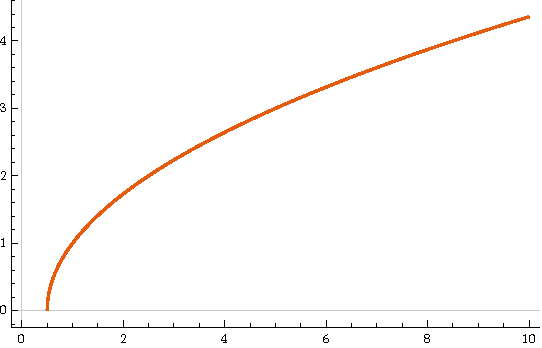
\includegraphics[width=10cm]{images/characteristic_curve.pdf}
  \end{center}
  Since $u\left( x,t \right)$ is constant along this characteristic curve, we must have $x_0 = x - \frac{1}{2}t^2$, and a solution of
  \begin{align*}
    u\left( x,t \right) &= u_0\left( x_0 \right)\\
                        &= u_0\left( x-\frac{1}{2}t^2 \right).
  \end{align*}
\end{example}
\begin{example}
  Consider now the equation
  \begin{align*}
    \pd{u}{t} + x\pd{u}{x} &= 0,
  \end{align*}
  with $u\left( x,0 \right) = x^2$. Solving $\diff{x}{t} = x$, we have
  \begin{align*}
    x(t) &= ce^{t}.
  \end{align*}
  We have $x(0) = c$, or that $x(t) = x_0e^{t}$. Using the fact that $u$ is constant along a characteristic, we have $x_0 = xe^{-t}$, and $u\left( x,t \right) = u_0\left( x_0 \right)$, giving
  \begin{align*}
    u\left( x,t \right) &= u_0\left( x_0 \right)\\
                        &= u_0\left( xe^{-t} \right)\\
                        &= x^2e^{-2t}.
  \end{align*}
\end{example}
Now, we ask ourselves when we may use the method of characteristics. Recall that there are three main types of linear partial differential equations:
\begin{itemize}
  \item Hyperbolic PDEs include the wave equation, and have two characteristic curves.
  \item Parabolic PDEs include the heat equation, and have one characteristic curve.
  \item Elliptic PDEs include Laplace's equation, and have no characteristic curves.
\end{itemize}
\begin{example}
  Consider
  \begin{align*}
    \pd{u}{t} + \frac{1}{t} \pd{u}{x} &= 0,
  \end{align*}
  with $u\left( x,0 \right) = \sin(x)$. Unfortunately, we can't use the method of characteristics to solve this equation. Instead, we may try
  \begin{align*}
    \pd{u}{t} + \frac{1}{t + 1}\pd{u}{x} &= 0,
  \end{align*}
  with the same initial condition. Then, 
  \begin{align*}
    \diff{x}{t} &= \frac{1}{t+1},
  \end{align*}
  so
  \begin{align*}
    x(t) &= \ln\left\vert t+1 \right\vert + c.
  \end{align*}
  Then, $x(0) = c$, so that
  \begin{align*}
    x(0) &= x - \ln\left\vert t+1 \right\vert.
  \end{align*}
  Yet again using the method of characteristics, we have
  \begin{align*}
    u\left( x,t \right) &= u_0\left( x_0 \right)\\
                        &= \sin\left( x-\ln\left\vert t+1 \right\vert \right)\\
                        &= \sin\left( x-\ln\left( t+1 \right) \right),
  \end{align*}
  as $t \geq 0$.
\end{example}
\begin{example}
  Consider
  \begin{align*}
    \pd{u}{t} + \left( x + t \right)\pd{u}{x} &= 0,
  \end{align*}
  with $u\left( x,0 \right) = \sin(x)$. We take
  \begin{align*}
    \diff{x}{t} &= x + t.
  \end{align*}
  We need an integrating factor to solve this problem.
\end{example}
\begin{example}
  Consider
  \begin{align*}
    \pd{u}{t} + t^2\pd{u}{x} &= 1,
  \end{align*}
  with $u\left( x,0 \right) = \sin(x)$. We're tempted to go ahead and try using the linearity principle, but before we try this, we recall how we created the characteristic curves in the first place, and write
  \begin{align*}
    1 &= \diff{u}{t}\\
      &= \pd{u}{t} + \diff{x}{t} \pd{u}{x}\\
      &= \pd{u}{t} + t^2\pd{u}{x}.
  \end{align*}
  This tells us that solutions propagate along characteristic curves, but along the curves, $u\left( x,t \right)$ increases at a constant rate of $1$.\newline

  We start by finding the characteristic curves:
  \begin{align*}
    \diff{x}{t}  &= t^2,
  \end{align*}
  so
  \begin{align*}
    x(t) &= \frac{1}{3}t^3 + x_0,
  \end{align*}
  or $x_0 = x - \frac{1}{3}t^3$. Therefore, we have
  \begin{align*}
    u\left( x,t \right) &= u_0\left( x_0 \right) + t\\
    &= u_0\left( x-\frac{1}{3}t^3 \right) + t,
  \end{align*}
  where $t$ is the addition that allows for $\diff{u}{t} = 1$. Plugging in our initial condition,
  \begin{align*}
    u\left( x,t \right) &= \sin\left( x - \frac{1}{3}t^3 \right) + t.
  \end{align*}
\end{example}
Recalling the transport equation,
\begin{align*}
  \pd{u}{t} + a \pd{u}{x} &= 0,
\end{align*}
this has the solution $u\left( x,t \right) = u_0\left( x-at \right)$. However, by making a slight tweak, we get Burgers's equation:
\begin{align*}
  \pd{u}{t} + u \pd{u}{x} &= 0,
\end{align*}
with solution $u\left( x,t \right) = u_0\left( x-ut \right)$.\footnote{Yes, this is an implicitly defined function.}
\subsection{Inhomogeneous Equations}%
We will tweak the standard heat equation:
\begin{align*}
  \pd{u}{t} &= k\pd{^2u}{x^2}
\end{align*}
by adding an inhomogeneous term,
\begin{align*}
  \pd{u}{t} &= k\pd{^2u}{x^2} + {\color{red} g(x)},
\end{align*}
defined on $0 \leq x \leq L$, $t\geq 0$, with boundary conditions of $u\left( 0,t \right) = a$, $u\left( L,t \right) = b$, and $u\left( x,0 \right) = f(x)$. We focus on functions of $x$ as our inhomogeneous term because otherwise it is too difficult.\footnote{According to Professor Miller, not even Mathematica could tackle this.} In order to solve this equation, we start by guessing\footnote{We have to do that again.} the equation is of the form
\begin{align*}
  u\left( x,t \right) &= v\left( x,t \right) + h\left( x \right),
\end{align*}

where $v$ is the homogeneous solution, and $h$ is some inhomogeneous term. 
\begin{enumerate}[(1)]
  \item The equation gives
  \begin{align*}
    \pd{u}{t} &= \pd{v}{t}\\
    \pd{^2u}{x^2} &= \pd{^2v}{x^2} + \diff{^2h}{x^2}.
  \end{align*}
  \item Plugging in the boundary conditions, we have
  \begin{align*}
    u\left( 0,t \right) &= v\left( 0,t \right) + h(0)\\
                        &= a\\
    u\left( L,t \right) &= v\left( L,t \right) + h(L)\\
                        &= b.
  \end{align*}
  \item Finally, with the initial condition, we have
  \begin{align*}
    u\left( x,0 \right) &= v\left( x,0 \right) + h\left( x \right).
  \end{align*}
\end{enumerate}
With the boundary conditions, we assume\footnote{This is different from guessing.} that $v\left( 0,t \right) = v\left( L,t \right) = 0$, so that $h\left( 0 \right) = a$ and $h\left( L \right) = b$. Plugging in our equation again, we must solve
\begin{align*}
  \pd{v}{t} &= k \pd{^2v}{x^2} + k\diff{^2h}{x^2} + g(x).
\end{align*}
This gives us two sub-problems:
\begin{enumerate}[(1)]
  \item We want to solve the Sturm--Liouville problem, 
    \begin{align*}
      \pd{v}{t} + k\pd{^2v}{x^2}
      \intertext{with}
      v\left( 0,t \right) &= 0\\
      v\left( L,t \right) &= 0\\
      v\left( x,0 \right) &= f(x) - h(x).
    \end{align*}
  \item We need to solve the one-dimensional boundary problem
    \begin{align*}
      k \diff{^2h}{x^2} + g(x) &= 0
      \intertext{with}
      h\left( 0 \right) &= a\\
      h\left( L \right) &= b.
    \end{align*}
\end{enumerate}
Solving the one-dimensional boundary problem, we may take
\begin{align*}
  \diff{^2h}{x^2} &= -\frac{1}{k}g(x)\\
  \diff{h}{x} &= -\frac{1}{k} \int_{}^{} g(x)\:dx + C\\
  h(x) &= -\frac{1}{k} \int_{}^{} \left( \int_{}^{} g(x)\:dx \right)\:dx + Cx + D.
\end{align*}
Here, the values of $C,D$ come from $a,b$. This allows us to know $h(x)$.\newline

Now, solving the Sturm--Liouville problem, we can go through the same arduous process to evaluate
\begin{align*}
  v\left( x,t \right) &= \sum_{n=1}^{\infty}A_ne^{-\frac{kn^2\pi^2}{L^2}t}\sin\left( \frac{n\pi }{L}x \right),
  \intertext{where}
  A_n &= \frac{2}{L} \int_{0}^{L} \left( f(x)-h(x) \right)\sin\left( \frac{n\pi }{L}x \right)\:dx.
\end{align*}
Therefore, we know $u\left( x,t \right) = v\left( x,t \right) + h(x)$.
\begin{example}
  We wish to solve
  \begin{align*}
    \pd{u}{t} + 2t \pd{u}{x} + 3t^2 \pd{u}{y} &= 0,
  \end{align*}
  where $u\left( x,y,0 \right) = x^2 + y^2$.\newline

  To solve this equation, we start by taking
  \begin{align*}
    \diff{}{t}\left( u\left( x(t),y(t),t \right) \right) &= \pd{u}{x}\diff{x}{t} + \pd{u}{y}\diff{y}{t} + \pd{u}{t}\\
                                                         &= 0.
  \end{align*}
  Matching coefficients, we get
  \begin{align*}
    \diff{x}{t} &= 2t\\
    \diff{y}{t} &= 3t^2.
  \end{align*}
  Therefore, we have
  \begin{align*}
    x-x_0 &= t^2\\
    y-y_0 &= t^3.
  \end{align*}
  Using the method of characteristics, we know that
  \begin{align*}
    u\left( x,y,t \right) &= u_0\left( x_0,y_0 \right)
  \end{align*}
  Therefore,
  \begin{align*}
    u_0\left( x_0,y_0 \right) &= x_0^2 + y_0^2.
  \end{align*}
  Manipulating our equations for $x_0$ and $y_0$, we have
  \begin{align*}
    x_0 &= x-t^2\\
    y_0 &= y-t^3,
  \end{align*}
  so that
  \begin{align*}
    u\left( x,y,t \right) &= \left( x-t^2 \right)^2 + \left( y-t^3 \right)^2.
  \end{align*}
  This is kind of boring. However, we are now able to solve an inhomogeneous equation:
  \begin{align*}
    \pd{u}{t} + 2t\pd{u}{x} + 3t^2 \pd{u}{y} &= y + t.
  \end{align*}
  Fixing our assumption with the inhomogeneous case, we have
  \begin{align*}
    \diff{}{t}\left( u\left( x(t),y(t),t \right) \right) &= \pd{u}{t} + 2t \pd{u}{x} + 3t^2 \pd{u}{y}\\
                                                         &= y + t.
  \end{align*}
  Integrating, we have
  \begin{align*}
    \int_{t_0}^{t} \diff{}{s}\left( u\left( x(s),y(s),s \right) \right)\:ds &= u\left( x(t),y(t),t \right) - u_0\left( x_0,y_0 \right)\\
                                                                            &= \int_{t_0}^{t} y(s) + s \:ds\\
                                                                            &= \int_{t_0}^{t} \left( y_0 + s^3 \right) + s\:ds\\
                                                                            &= y_0s + \frac{1}{4}s^4 + \frac{1}{2}s^2\biggr\vert_{t_0}^{t}.
                                                                            \intertext{Assuming $t_0 = 0$ and plugging in our definition of $y_0 = y-t^3$}
                                                                            &= \left( y-t^3 \right)t + \frac{1}{4}t^3 + \frac{1}{2}t^2.
  \end{align*}
  
\end{example}
\subsection{Degrees of Linearity}%
Considering all first-order partial differential equations, only a small subset of these equations are linear. We want to try to understand the general case of first-order equations.
\begin{definition}
  A \textit{general} first-order PDE in $2$ variables is of the form
  \begin{align*}
    F\left( x,y, u, \pd{u}{x}, \pd{u}{y}\right) &= 0.
  \end{align*}
\end{definition}
\begin{definition}
  A \textit{quasilinear} first-order PDE in $2$ variables is of the form
  \begin{align*}
    a\left( x,y,u \right) \pd{u}{x} + b\left( x,y,u \right) \pd{u}{y} &= c\left( x,y,u \right).
  \end{align*}
  A quasilinear second-order PDE in $2$ variables is of the form
  \begin{align*}
    a\left( x,y,u,\pd{u}{x},\pd{u}{y} \right) \pd{^2u}{x^2} + b\left( x,y,u,\pd{u}{x},\pd{u}{y} \right) \pd{^2u}{x\partial y} + c\left( x,y,u,\pd{u}{x},\pd{u}{y} \right) \pd{^2u}{y^2} &= d\left( x,y,u,\pd{u}{x}, \pd{u}{y} \right).
  \end{align*}
\end{definition}
It is pretty clear that these get out of hand really quickly.
\begin{definition}
  A \textit{semilinear} first-order PDE in $2$ variables is of the form
  \begin{align*}
    a\left( x,y \right) \pd{u}{x} + b\left( x,y \right) \pd{u}{y} &= c\left( x,y,u \right).
  \end{align*}
\end{definition}
\begin{example}
  Consider the equation
  \begin{align*}
    \left( x+y \right)\pd{u}{x} + \left( x-y \right)\pd{u}{y} &= 3u.\label{eq:hard_pde}\tag{\textasteriskcentered}
  \end{align*}
  This is a first-order linear equation. Rewriting
  \begin{align*}
    \pd{u}{x} + \frac{x-y}{x+y}\pd{u}{y} &= \frac{3}{x+y} u.
  \end{align*}
  Therefore,
  \begin{align*}
    \diff{y}{x} &= \frac{x-y}{x+y}.
  \end{align*}
  This is not a linear ODE.\newline

  Considering the linear equation
  \begin{align*}
    3\pd{u}{x} + 5\pd{u}{y} &= 2u,
  \end{align*}
  which we may put into ``standard form''
  \begin{align*}
    \pd{u}{x} + \frac{5}{3}\pd{u}{y} &= \frac{2}{3}u
  \end{align*}
  Then, we are able to use the method of characteristics, taking
  \begin{align*}
    \diff{}{x}\left( u\left( x,y \right) \right) &+ \pd{u}{x} + \pd{u}{y}\diff{y}{x}\\
                                                 &= \frac{2}{3}u,
  \end{align*}
  which means $\diff{y}{x} = \frac{5}{3}$, and $\diff{u}{x} = \frac{2}{3}u$. \newline

  Solving
  \begin{align*}
    \diff{u}{x} &= \frac{2}{3}u,
  \end{align*}
  we get
  \begin{align*}
    \ln\left\vert \frac{u}{u_0} \right\vert &= \frac{2}{3}\left( x-x_0 \right).
  \end{align*}
  and solving
  \begin{align*}
    \diff{y}{x} &= \frac{5}{3},
  \end{align*}
  we get
  \begin{align*}
    y-y_0 &= \frac{5}{3}\left( x-x_0 \right).
  \end{align*}
  Via the method of characteristics, and noting that our equation $\diff{u}{x} = \frac{2}{3}u$ is not homogeneous, we have
  \begin{align*}
    u\left( x,y \right) &= u_0\left( x_0.y_0 \right) + \frac{2}{3}\left( x-x_0 \right),
  \end{align*}
  Inputting an initial condition, $u_0\left( x,y \right) = x + y^2$, we need to find $x_0$ and $y_0$. This is still not fun.\newline

  As it turns out, we need to use a special version of the method of characteristics that does not favor either variable.
\end{example}
\begin{example}
  Considering again the transport equation,
  \begin{align*}
    \pd{u}{t} + 3 \pd{u}{x} &= 0,
  \end{align*}
  and
  \begin{align*}
    \diff{u}{t} &= \pd{u}{t} + \diff{x}{t} \pd{u}{t},
  \end{align*}
  we try to see if we can write this in more linear-algebraic terms. Writing
  \begin{align*}
    \pd{u}{t} + \pd{u}{x}\diff{x}{t} - \diff{u}{t} &= 0\\
    \left( 1 \right) \left( \pd{u}{t} \right) + \pd{u}{x}\diff{x}{t} - \left( 1 \right) \diff{u}{t} &= 0.
  \end{align*}
  We may write this equation as
  \begin{align*}
    \begin{pmatrix}\pd{u}{t}\\ \pd{u}{x} \\ -1 \end{pmatrix} \cdot \begin{pmatrix}1\\ \diff{x}{t} \\ \diff{u}{t}\end{pmatrix} &= 0.
  \end{align*}
  We need some concepts from multivariable calculus. Recall that if we have a vector-valued function
  \begin{align*}
    \mathbf{f}\left( t \right) &= \begin{pmatrix}3\cos\left( t \right)\\ 2\sin\left( t \right)\\t\end{pmatrix},
  \end{align*}
  the tangent vector is defined as the derivative
  \begin{align*}
    \diff{\mathbf{f}}{t} &= \begin{pmatrix}-3\sin\left( t \right)\\2\cos\left( t \right)\\1\end{pmatrix}.
  \end{align*}
  Similarly, in higher dimensions, we may consider characteristic \textit{surfaces}.
\end{example}
In general, the method of characteristics requires us to integrate an initial function, which becomes the solution function. For instance, using the method of characteristics, we may solve the wave equation
\begin{align*}
  \pd{^2u}{t^2} - c^2 \pd{^2u}{x^2}&= 0
\end{align*}
with initial conditions of $u\left( x,0 \right) = f(x)$ and $\pd{u}{t}\bigr\vert_{(x,0)} = g(x)$ by taking
\begin{align*}
  u\left( x,t \right) &= \frac{1}{2}\left( f\left( x-ct \right) + f\left( x+ct \right) \right) + \frac{1}{2c} \int_{x-ct}^{x+ct} g(s)\:ds.\label{eq:dalembert_solution}\tag{\textdagger}
\end{align*}
\begin{example}
  Recall that
  \begin{align*}
    \pd{^2u}{x^2} - a^2\pd{^2u}{x^2} &= 0
  \end{align*}
  can be rewritten as
  \begin{align*}
    \left( \pd{}{t} - a\pd{}{x} \right) \left( \pd{}{t}+ a\pd{}{x} \right) u &= 0
  \end{align*}
  Similarly, we are able to split up
  \begin{align*}
    \pd{^2u}{x^2} + \pd{^2u}{y^2} &= 0,
  \end{align*}
  to obtain
  \begin{align*}
    \left( \pd{}{x} + i \pd{}{y} \right)\left( \pd{}{x} - i \pd{}{y} \right) u &= 0.
  \end{align*}
\end{example}
The equation \eqref{eq:dalembert_solution} is known as D'Alembert's solution to the wave equation. Generally, deriving the solution requires a change of coordinates by using the Jacobian to change $\eta = x - at$ and $\xi = x + at$, and then taking
\begin{align*}
  \pd{^2}{\xi\partial\eta }u\left( \xi,\eta \right) &= 0.
\end{align*}
This sucks, though.\newline

To obtain D'Alembert's solution, we start by noting that
\begin{align*}
  u\left( x,t \right) &= c_1\left( x-at \right) + c_2\left( x + at \right)
\end{align*}
does solve the wave equation. We insert functions $h$ and $k$ to take the equation
\begin{align*}
  u\left( x,t \right) &= h\left( x-at \right) + k\left( x + at \right).
\end{align*}
Inserting the initial conditions, we have
\begin{align*}
  u\left( x,0 \right) &= h(x) + k(x)\\
                      &= f(x)\\
                      \\
  \pd{u}{t}\biggr\vert_{(x,0)} &= -a \pd{h}{t}\biggr\vert(x,0) + a \pd{k}{t}\biggr\vert_{(x,0)}\\
                               &= -a\diff{h}{x} + a\diff{k}{x}\\
                               &= g(x).
\end{align*}
Now, we integrate the second equation and multiply the expression $h(x) + k(x) = f(x)$, giving
\begin{align*}
  -a h(x) + ak(x) &= \int_{x_0}^{x} g(s)\:ds\\
  ah(x) + ak(x) &= af(x).
\end{align*}
Adding and subtracting, we get the expressions
\begin{align*}
  2ak(x) &= af(x) + \int_{x_0}^{x} g(s)\:ds\\
  2ah(x) &= af(x) - \int_{x_0}^{x} g(s)\:ds.
\end{align*}
Therefore, we get
\begin{align*}
  k(x) &= \frac{1}{2}f(x) + \frac{1}{2a}\int_{x_0}^{x} g(s)\:ds\\
  h(x) &= \frac{1}{2}f(x) - \frac{1}{2a} \int_{x_0}^{x} g(s)\:ds.
\end{align*}
Substituting, we have
\begin{align*}
  u\left( x,t \right) &= \frac{1}{2} \left( f(x-at) + f(x + at) \right) + \int_{x_0}^{x+at} g(s)\:ds - \int_{x_0}^{x-at} g(s)\:ds\\
                      &= \frac{1}{2}\left( f(x-at) + f(x+at) \right) + \int_{x-at}^{x + at} g(s)\:ds.
\end{align*}
\begin{example}
  Suppose we have the wave equation
  \begin{align*}
    \pd{^2u}{t^2} &= 4\pd{^2u}{x^2},
  \end{align*}
  with $u\left( x,0 \right) = x^2$ and $\pd{u}{t}\bigr\vert_{(x,0)} = g(x)$. Then, we have the solution
  \begin{align*}
    u\left( x,t \right) &= \frac{1}{2}\left( \left( x-2t \right)^2 + \left( x + 2t \right)^2 \right) + \frac{1}{4}\int_{x-2t}^{x+2t} \cos\left( s \right)\:ds\\
                        &= 2x^2 + 8t^2 + \frac{1}{4}\left( \sin\left( x+2t \right) - \sin\left( x - 2t \right) \right).
  \end{align*}
\end{example}
\begin{example}
  Consider
  \begin{align*}
    \pd{^2u}{t^2} - 5 \pd{^2u}{x\partial t} - 14 \pd{^2u}{x^2} &= 0,
  \end{align*}
  with $u\left( x,0 \right) = f(x)$ and $\pd{u}{t}\bigr\vert_{(x,0)} = g(x)$ .Then, we may write this as
  \begin{align*}
    \left( \pd{}{t} - 7 \pd{}{x} \right) \left( \pd{}{t} + 2 \pd{}{x} \right) u &= 0.
  \end{align*}
  We have the characteristic curves of $x-7t$ and $x + 2t$.\newline

  Reworking our derivation of D'Alembert's solution, we have
  \begin{align*}
    u\left( x,t \right) &= h\left( x + 7t \right) + k\left( x-2t \right).
  \end{align*}
  We have
  \begin{align*}
    u\left( x,0 \right) &= h(x) + k(x)\\
    \pd{u}{t}\biggr\vert_{(x,0)} &= 7\diff{h}{x} - 2 \diff{k}{x}.
  \end{align*}
  This gives
  \begin{align*}
    h(x) + k(x) &= f(x)\\
    7 \diff{h}{x} - 2 \diff{k}{x} &= g(x)\\
    7h(x) -2k(x) &= \int_{x_0}^{x} g(s)\:ds.
  \end{align*}
  After much suffering, we have
  \begin{align*}
    u\left( x,t \right) &= \frac{2}{9}f\left( x + 7t \right) + \frac{7}{9}f\left( x-2t \right) + \frac{1}{9} \int_{x-2t}^{x+7t} g(s)\:ds.
  \end{align*}
\end{example}
\begin{example}
  Consider the equation
  \begin{align*}
    \pd{^2u}{t^2} + \pd{^2u}{x^2} &= 0,
  \end{align*}
  with $-\infty < x < \infty$ and $t\geq 0$. This gives
  \begin{align*}
    \left( \pd{}{t} + i \pd{}{x} \right) \left( \pd{}{t} - i \pd{}{x} \right) u &= 0.
  \end{align*}
\end{example}
\begin{example}
  Consider the equation
  \begin{align*}
    \pd{^2u}{t^2} - x^2 \pd{^2u}{x^2} &= 0.
  \end{align*}
  Factoring, we take
  \begin{align*}
    \left( \pd{}{t} - x\pd{}{x} \right) \left( \pd{}{t} + x \pd{}{x} \right) u &= 0.
  \end{align*}
  As it turns out, this doesn't work --- it's not so simple (use product rule).
\end{example}
\begin{example}
  Consider the equation
  \begin{align*}
    t \pd{u}{t} &= x \pd{u}{x},
  \end{align*}
  with initial condition $u\left( x,0 \right) = \frac{2}{x^2 + 1}$.\newline

  Putting it in ``standard form,'' we have
  \begin{align*}
    \pd{u}{t} - \frac{x}{t} \pd{u}{x} &= 0.
  \end{align*}
  Therefore,
  \begin{align*}
    \diff{x}{t} &= -\frac{x}{t}.
  \end{align*}
  Separating variables, we have
  \begin{align*}
    \frac{dx}{x} &= -\frac{dt}{t},
  \end{align*}
  so
  \begin{align*}
    \ln\left( x \right)-\ln\left( x_0 \right) &= \ln\left(t_0  \right) - \ln\left( t \right).
  \end{align*}
  This is not good. We may change the initial condition to set, $u\left( x,2 \right) = \frac{2}{x^2 + 1}$. This gives
  \begin{align*}
    \ln\left( xt \right) - \ln\left( 2x_0 \right) &= 0,
  \end{align*}
  so $x_0 = \frac{xt}{2}$. Thus,
  \begin{align*}
    u\left( x,t \right) &= u_0\left( x_0 \right)\\
                        &= \frac{2}{x_0^2 + 1}\\
                        &= \frac{8}{\left( xt \right)^2 + 4}
  \end{align*}
\end{example}
\begin{example}
  Consider the equation
  \begin{align*}
    \pd{u}{t} + \left( x + t \right)\pd{u}{x} &= 4,
  \end{align*}
  with initial condition $u\left( x,0 \right) = \ln\left( x^2 + 1 \right)$.\newline

  Thus,
  \begin{align*}
    \diff{x}{t} &= x + t.
  \end{align*}
  This is an issue. We guess
  \begin{align*}
    x(t) &= Ae^{t} + Bt + C.
  \end{align*}
  Knowing that $t_0 = 0$, we have
  \begin{align*}
    x(t) &= \left( x_0 - C \right)e^{t} + Bt + C.
  \end{align*}
  Furthermore, we know that
  \begin{align*}
    \diff{x}{t} &= Ae^{t} + B,
  \end{align*}
  so
  \begin{align*}
    \diff{x}{t} - x &= \left( B-C \right) - Bt,
  \end{align*}
  meaning $B = -1$, and $C = -1$. Thus,
  \begin{align*}
    x(t) &= Ae^{t} - t - 1.
  \end{align*}
  Therefore,
  \begin{align*}
    x_0 &= A-1.
  \end{align*}
  This gives
  \begin{align*}
    x(t) &= \left( x_0 + 1 \right)e^{t} - t - 1.
  \end{align*}
  Therefore,
  \begin{align*}
    \left( x+ t+ 1 \right)e^{-t} &= x_0 + 1,
  \end{align*}
  and
  \begin{align*}
    x_0 &= \left( x + t + 1 \right)e^{-t} - 1.
  \end{align*}
  We are tempted to say that $u\left( x,t \right) = u_0\left( x_0 \right)$; unfortunately, we need one more thing. Recall that the method of characteristics says
  \begin{align*}
    \diff{u}{t} &= \pd{u}{t} + \pd{u}{x}\diff{x}{t}\\
                &= 4,
  \end{align*}
  so integrating,
  \begin{align*}
    u\left( x,t \right) - u_0\left( x_0 \right) &= 4t\\
    u\left( x,t \right) &= \ln\left( \left( \left( x + t + 1 \right)e^{-t} - 1 \right)^2 + 1 \right) + 4t.
  \end{align*}
\end{example}
\begin{example}
  Consider the equation
  \begin{align*}
    x\pd{u}{t} + t\pd{u}{x} &= 0,
  \end{align*}
  with $u\left( x,0 \right) = \cos\left( x \right)$. Writing in standard form, we have
  \begin{align*}
    \pd{u}{t} + \frac{t}{x} \pd{u}{x} &= 0,
  \end{align*}
  so that
  \begin{align*}
    \diff{x}{t} &= \frac{t}{x}.
  \end{align*}
  Separating variables and solving, we have
  \begin{align*}
    \frac{x^2}{2} - \frac{x_0^2}{2} &= \frac{t^2}{2}.
  \end{align*}
  Multiplying out,
  \begin{align*}
    x_0^2 &= x^2 - t^2,
  \end{align*}
  so
  \begin{align*}
    x_0 &= \sqrt{x^2 - t^2}.
  \end{align*}
  Thus,
  \begin{align*}
    u\left( x,t \right) &= u_0\left( x_0 \right)\\
                        &= \cos\left( \sqrt{x^2 - t^2} \right)
  \end{align*}
  At first glance, we're done, but we're not. Note that $\sqrt{x^2 - t^2}$ is real whenever $x^2 \geq t^2$, meaning we need to restrict our domain. Note that if $x^2 < t^2$, our cosine turns into a hyperbolic cosine, so our solution is actually unbounded.
\end{example}
\begin{example}
  Recall Burgers's equation,
  \begin{align*}
    \pd{u}{t} + u \pd{u}{x} &= 0,\label{eq:burgers_equation}\tag{$\ddag$}
  \end{align*}
  with $u\left( x,0 \right) = \sin\left( x \right)$. This is actually known as Burgers's \textit{inviscid} equation --- in the general Burgers equation, there is a viscosity term.\newline

  When we solved this equation before, we obtained
  \begin{align*}
    u\left( x,t \right) &= \sin\left( x-u t \right).
  \end{align*}
  We may also generalize \eqref{eq:burgers_equation} by taking
  \begin{align*}
    \pd{u}{t} + \pd{}{x}\left( f(u) \right) &= 0.
  \end{align*}
  Now, these equations are equal to each other if and only if
  \begin{align*}
    f(u) &= \frac{u^2}{2}.
  \end{align*}
\end{example}
\section{Hyperbolic Systems}%
Let
\begin{align*}
  \mathbf{u} &= \begin{pmatrix}u_1\left( x,t \right)\\u_2\left( x,t \right)\end{pmatrix},
\end{align*}
and
\begin{align*}
  \mathbf{f}\left( \mathbf{u} \right) &= \begin{pmatrix}f_1\left( \mathbf{u} \right)\\ f_2\left( \mathbf{u} \right)\end{pmatrix}\\
                                      &= \begin{pmatrix} f_1\left( u_1,u_2 \right)\\ f_2\left( u_1,u_2 \right)\end{pmatrix}.
\end{align*}
Then, the ``derivative'' of $\mathbf{f}$ is the Jacobian of $\mathbf{f}$.\newline

Now, if the eigenvalues of $\diff{\mathbf{f}}{\mathbf{u}}$ are real and $\diff{\mathbf{f}}{\mathbf{u}}$ is diagonalizable, then
\begin{align*}
  \pd{\mathbf{u}}{t} + \diff{\mathbf{f}}{\mathbf{u}}\pd{\mathbf{u}}{x} &= 0
\end{align*}
is known as a \textit{hyperbolic system}.
\begin{example}
  Consider
  \begin{align*}
    \mathbf{u} &= \begin{pmatrix}v\left( x,t \right)\\ w\left( x,t \right)\end{pmatrix}\\
    \mathbf{f}\left( \mathbf{u} \right) &= \begin{pmatrix}vw^2 \\ w + 2v\end{pmatrix}.
  \end{align*}
  Then,
  \begin{align*}
    \diff{\mathbf{f}}{\mathbf{u}} &= \begin{pmatrix}w^2 & 2vw \\ 2 & 1\end{pmatrix}
  \end{align*}
  Finding the eigenvalues, we have
  \begin{align*}
    \det\left( A - \lambda I \right) &= \left( w^2 -\lambda \right)\left( 1-\lambda \right) - 4vw\\
                                     &= 0,
  \end{align*}
  so that
  \begin{align*}
    \lambda^2 + \left( w^2 - 1 \right)\lambda + w^2 - 4vw &= 0,
  \end{align*}
  meaning
  \begin{align*}
    \lambda &= \frac{\left( 1-w^2 \right)\pm \sqrt{\left( w^2 - 1 \right)^2 - 4\left( 4w^2-4vw \right)}}{2}.
  \end{align*}
  Now, if
  \begin{align*}
    \left( w^2 - 1 \right)^2 - 4\left( w^2 - 4vw \right) &> 0,
  \end{align*}
  then this is a hyperbolic system.
\end{example}
\begin{example}
  Consider the general system
  \begin{align*}
    \mathbf{w} &= \begin{pmatrix}u\left( x,t \right)\\ v\left( x,t \right)\end{pmatrix}\\
    \mathbf{w}_0 &= \begin{pmatrix}u\left( x,0 \right)\\ v\left( x,0 \right)\end{pmatrix}\\
    \pd{\mathbf{w}}{t} &= A \pd{\mathbf{w}}{x},
  \end{align*}
  where $A$ is a constant coefficient matrix. Now, if $A$ is diagonalizable, we want the matrix $P$ such that $PDP^{-1} = A$ so that we may decouple this system.\newline

  Afterwards, we will define a change of coordinates
  \begin{align*}
    \mathbf{z} &= \begin{pmatrix}z_1\left( x,t \right) \\ z_2\left( x,t \right)\end{pmatrix}.
  \end{align*}
  We will let
  \begin{align*}
    \mathbf{z} &= P^{-1}\mathbf{w}.
  \end{align*}
  Taking
  \begin{align*}
    \pd{\mathbf{z}}{t} &= P^{-1} \pd{\mathbf{w}}{t}\\
                       &= P^{-1}A \pd{\mathbf{w}}{x}\\
                       &= P^{-1}\left( PDP^{-1} \right) \pd{\mathbf{w}}{x}\\
                       &-= DP^{-1} \pd{\mathbf{w}}{x}\\
                       &= D \pd{\mathbf{z}}{x}.
  \end{align*}
  This is our decoupled system.\newline

  Finally,
  \begin{align*}
    \mathbf{z}_0 &= P^{-1} \mathbf{w}_0
  \end{align*}
  This will give the solution
  \begin{align*}
    \mathbf{w}\left( x,t \right) &= P \mathbf{z}\left( x,t \right).
  \end{align*}
  
\end{example}
\begin{example}
  In the case with
  \begin{align*}
    A &= \begin{pmatrix}4 & -3 \\ 7 & -6\end{pmatrix}\\
    \mathbf{w}_0 &= \begin{pmatrix}e^x\\x^2\end{pmatrix},
  \end{align*}
  we want to find the eigenvalues and eigenvectors. Using some black magic, we can obtain
  \begin{align*}
    \lambda_1 &= 1\\
    \mathbf{v}_1 &= \begin{pmatrix}1\\1\end{pmatrix}\\
    \lambda_2 &= -3\\
    \mathbf{v}_2 &= \begin{pmatrix}3\\7\end{pmatrix}.
  \end{align*}
  Therefore,
  \begin{align*}
    P &= \begin{pmatrix}1 & 3 \\ 1 & 7\end{pmatrix}\\
    P^{-1} &= \frac{1}{4} \begin{pmatrix}7 & -3 \\ -1 & 1\end{pmatrix}\\
    D &= \begin{pmatrix}1 & 0 \\ 0 & -3\end{pmatrix}.
  \end{align*}
  We take
  \begin{align*}
    \mathbf{z}_0 &= P^{-1} \begin{pmatrix}e^{x}\\x^2\end{pmatrix}\\
                 &= \frac{1}{4} \begin{pmatrix}7e^{x} - 3x^2\\ -e^{x} + x^2\end{pmatrix}.
  \end{align*}
  Writing the decoupled system, we get
  \begin{align*}
    \pd{z_1}{t} &= \pd{z_1}{x}\\
    \pd{z_2}{t} &= -3\pd{z_2}{x},
  \end{align*}
  with
  \begin{align*}
    z_1\left( x,0 \right) &= \frac{1}{4}\left( 7e^{x} - 3x^2 \right)\\
    z_2\left( x,0 \right) &= \frac{1}{4}\left( -e^{x} + x^2 \right)
  \end{align*}
  Both of these are just transport equations. Therefore,
  \begin{align*}
    z_1\left( x,t \right) &= \frac{1}{4}\left( 7e^{x + t} - 3\left( x+t \right)^2 \right)\\
    z_2\left( x,t \right) &= \frac{1}{4}\left( -e^{x - 3t} + \left( x-3t \right)^2 \right)
  \end{align*}
  Therefore, we have the solution
  \begin{align*}
    \mathbf{w}\left( x,t \right) &= \frac{1}{4} \begin{pmatrix}1 & 3 \\ 1 & 7\end{pmatrix} \begin{pmatrix}7e^{x + t} - 3\left( x +t \right)^2\\ -e^{x-3t} + \left( x-3t \right)^2\end{pmatrix}\\
                                 &= \frac{1}{4} \begin{pmatrix}7e^{x+t} - 3\left( x + t \right)^2 - e^{x-3t} + \left( x-3t \right)^2 \\ 21e^{x + t} - 9\left( x + t \right)^2 - 7e^{x-3t} + 7\left( x-3t \right)^2\end{pmatrix}
  \end{align*}
\end{example}
\begin{example}
  Consider the equation
  \begin{align*}
    \pd{u}{t} + \pd{u}{x} + \pd{u}{y} &= u,
  \end{align*}
  with $u\left( x,y,0 \right) = xe^{y}$. Then, via the method of characteristics,
  \begin{align*}
    \diff{x}{t} &= 1\\
    \diff{y}{t} &= 1\\
    \diff{u}{t} &= u.
  \end{align*}
  {\color{red}Note that
  \begin{align*}
    \diff{u}{t} &\neq \pd{u}{t}.
  \end{align*}}
  Now, solving our equations using $t_0 = 0$, we get
  \begin{align*}
    x-x_0 &= t\\
    y-y_0 &= t\\
    u\left( x,y,t \right) &= u\left( x,y,0 \right)e^{t}.
  \end{align*}
  Thus, we get
  \begin{align*}
    u\left( x,y,t \right) &= u_0\left( x_0,y_0 \right)e^{t}\\
                          &= x_0e^{y_0}e^{t}\\
                          &= \left( x-t \right)e^{y-t}e^{t}\\
                          &= \left( x-t \right)e^{y}.
  \end{align*}
  Let's verify this. We calculate
  \begin{align*}
    u\left( x,y,0 \right) &= xe^{y}\\
    \pd{u}{t} &= -e^{y}\\
    \pd{u}{x} &= e^{y}\\
    \pd{u}{y} &= \left( x-t \right)e^{y}.
  \end{align*}
  Thus, this is actually a solution.
\end{example}
\section{Integral Transforms}%
Integral transforms are a way to convert differential equations to other classes of equations.\newline

For instance, the Laplace transform, defined by
  \begin{align*}
    \mathcal{L}\left[ f(t) \right] &= \int_{0}^{\infty} e^{-st}f(t)\:dt,
  \end{align*}
  is an integral transform.
\begin{example}
  Consider 
  \begin{align*}
    f(t) &= e^{3t}.
  \end{align*}
  Then, so long as $s > 3$, we have
  \begin{align*}
    \mathcal{L}\left[ f(t) \right] &= \int_{0}^{\infty} e^{\left( 3-s \right)t}\:dt\\
                                   &= \frac{1}{3-s}e^{\left( 3-s \right)t}\biggr\vert_{t=0}^{\infty}\\
                                   &= \frac{1}{s-3}
  \end{align*}
  Generally, as long as $s > a$,
  \begin{align*}
    \mathcal{L}\left[ e^{at} \right] &= \frac{1}{s-a}.
  \end{align*}
\end{example}
\begin{example}
  If $F(s) = \mathcal{L}\left[ f(t) \right]$, then, assuming $\diff{f}{t}$ is integrable over $[0,\infty)$ and $s > 0$,
  \begin{align*}
    \mathcal{L}\left[ \diff{f}{t} \right] &= \int_{0}^{\infty} e^{-st}\diff{f}{t}\:dt\\
                                          &= f(t)e^{-st}\biggr\vert_{0}^{\infty} - \left( -s \right) \int_{0}^{\infty} e^{-st}f(t)\:dt\\
                                          &= -f(0) + s\int_{0}^{\infty} e^{-st}f(t)\:dt\\
                                          &= -f(0) + sF(s).
  \end{align*}
\end{example}
\begin{definition}
  If $f(t)$ is a function, then an \textit{integral transform} of $f$ is a function
  \begin{align*}
    F(s) &= \int_{a}^{b} K\left( s,t \right)f(t)\:dt.
  \end{align*}
  This expression yields
  \begin{align*}
    f(t) &= \int_{c}^{d} K^{\ast}\left( t,s \right)F(s)\:ds,
  \end{align*}
  where $K^{\ast}\left( t,s \right)$ is the dual of $K\left( s,t \right)$.
\end{definition}
In an integral transform, $K\left( s,t \right)$, $a$, and $b$ uniquely identify the transform.\newline

Now, when we learned the Laplace transform back in ODEs, we did not discuss the inverse of the Laplace transform. Unfortunately, the inverse Laplace transform requires integration in the complex plane.\footnote{We discussed the residue theorem (but not the inverse Laplace transform itself) in depth in \href{https://ai.avinash-iyer.com/Classes_and_Homework/College/Y4/Y4S2,\%20Math\%20Methods\%20II/math_methods_2_notes.pdf}{Math Methods 2}.} The inverse Laplace transform itself is
\begin{align*}
  f(t) &= \int_{\gamma - i\infty}^{\gamma + i\infty} e^{st}F(s)\:ds.
\end{align*}
Here, we choose the value of $\gamma$ such that the integral converges. Usually, we choose to use a table in order to use the inverse Laplace transform.\newline

Let's introduce a new integral transform.
\begin{definition}
  Given $f(t)$ absolutely integrable over $\R$, we define
  \begin{align*}
    \hat{f}\left( \omega \right) &= \mathcal{F}\left[ f(t) \right]\\
                                 &= \int_{-\infty}^{\infty} e^{i\omega t}f(t)\:dt.\label{eq:fourier_transform}\tag{$\dag$}
  \end{align*}
  Here, $a = \infty$, $b = -\infty$, and $K\left( \omega,t \right) = e^{i\omega t}$.
\end{definition}
\begin{definition}
  The \textit{inverse Fourier transform} of $\hat{f}\left( \omega \right)$ is
  \begin{align*}
    f(t) &= \frac{1}{2\pi} \int_{-\infty}^{\infty} e^{-i\omega t}\hat{f}\left( \omega \right)\:d\omega.
  \end{align*}
\end{definition}
\begin{remark}
  There are other versions of the Fourier transform (mostly dependent on the sign of $i\omega t$ or where the $2\pi$ goes). For instance, in \href{https://ai.avinash-iyer.com/Classes_and_Homework/College/Y4/Y4S1,\%20Math\%20Methods/math_methods_notes.pdf}{Math Methods}, we used
  \begin{align*}
    \hat{f}\left( \omega \right) &= \frac{1}{\sqrt{2\pi}} \int_{-\infty}^{\infty} e^{-i\omega t}f(t)\:dt.
  \end{align*}
  For this class, we will use the definition in \eqref{eq:fourier_transform}.
\end{remark}
The Fourier transform essentially takes a signal in time, and decomposes the signal into its frequencies.
\begin{example}
  Consider the standard normal distribution,
  \begin{align*}
    p(t) &= \frac{1}{\sqrt{2\pi}\sigma} e^{\frac{-\left( t-\mu \right)^2}{2\sigma^2}}.
  \end{align*}
  Then,
  \begin{align*}
    \int_{-\infty}^{\infty} p(t)\:dt &= 1,
  \end{align*}
  and $p(t) \geq 0$ for all $t$, so $p(t)$ is a probability distribution.\newline

  The standard deviation of the probability distribution $p(t)$ is equal to the distance between the two inflection points of the distribution.\newline

  Now, suppose we start taking $\sigma\rightarrow 0$. We must always maintain the condition that
  \begin{align*}
    \int_{}^{} \frac{1}{\sqrt{2\pi}\sigma}e^{\frac{-\left( t-\mu \right)^2}{2\sigma^2}}\:dt &= 1,
  \end{align*}
  which holds for all $\sigma > 0$ and for all $\mu\in\R$. We may define
  \begin{align*}
    \delta\left( t-\mu \right) &= \lim_{\sigma\rightarrow 0} p(t).
  \end{align*}
  This is known as the \textit{Dirac delta distribution}.\newline

  We use the delta distribution to model ``impulse forces'' that basically only exist at one point.
\end{example}
\begin{definition}
  The following are the three principles of the delta distribution.
  \begin{enumerate}[(a)]
    \item 
      \begin{align*}
        \int_{-\infty}^{\infty} \delta\left( t-\mu \right)\:dt &=1.
      \end{align*}
    \item If $\Theta(t)$ is the \href{https://en.wikipedia.org/wiki/Heaviside_step_function}{Heaviside step function}
      \begin{align*}
        \diff{}{t}\left( \theta(t) \right) &= \delta(t).
      \end{align*}
    \item 
      \begin{align*}
        \int_{-\infty}^{\infty} f(s)\delta(s)\:ds &= 0.
      \end{align*}
  \end{enumerate}
\end{definition}
\begin{example}
  Consider
  \begin{align*}
    f(t) &= \sin\left( 5t \right).
  \end{align*}
  Then,
  \begin{align*}
    \hat{f}\left( \omega \right) &= ic\left( \delta\left(\omega - 5\right) - \delta\left( \omega + 5 \right) \right).
  \end{align*}
  Here, $c$ is a constant that depends on how we define the Fourier transform.
\end{example}
\begin{example}
  How might we solve a differential equation using the Fourier transform?\newline

  If $f(t)$ is a sufficiently well-behaved function,\footnote{Depending on the field, we're discussing either \href{https://en.wikipedia.org/wiki/Schwartz_space}{Schwartz functions}, square-integrable functions, or absolutely integrable functions.} then
  \begin{align*}
    \hat{f}\left( \omega \right) &= \int_{-\infty}^{\infty} e^{i\omega t}f(t)\:dt\\
    f(t) &= \frac{1}{2\pi}\int_{-\infty}^{\infty} e^{-i\omega t}\hat{f}(\omega)\:d\omega.
  \end{align*}
  If $f$ is well-behaved (by our desired criterion) and its derivative is sufficiently well-behaved (by the same criterion),\footnote{Note that by our definition of ``sufficiently well-behaved,'' $\lim_{t\rightarrow\pm\infty}f(t) = 0$.} then by integrating by parts,
  \begin{align*}
    \mathcal{F}\left[ \diff{f}{t} \right] &= \int_{-\infty}^{\infty} e^{i\omega t}\diff{f}{t}\:dt\\
                                          &= \left( f(t)e^{i\omega t} \right)\biggr\vert_{-\infty}^{\infty} -i\omega \int_{-\infty}^{\infty} e^{i\omega t}f(t)\:dt\\
                                          &= -i\omega \mathcal{F}\left[ f \right].
  \end{align*}
  In general,
  \begin{align*}
    \mathcal{F}\left[ \diff{^nf}{t^n} \right] &= \left( -i\omega \right)^{n} \mathcal{F}\left[ f \right].
  \end{align*}
\end{example}
\begin{table}[t]
  \centering
  \renewcommand{\arraystretch}{2}
  \begin{tabular}{c|c}
    $ f(t) = \frac{1}{2\pi} \int_{-\infty}^{\infty} e^{-i\omega t}\hat{f}(\omega)\:d\omega$ & $ \hat{f}(k) = \int_{-\infty}^{\infty} e^{i\omega t}f(t)\:dt$\\
    \hline\hline
    $\displaystyle \diff{f}{t}$ & $\displaystyle -i\omega \hat{f}\left( \omega \right)$\\
    $\displaystyle \diff{^{n}f}{t^{n}}$ & $\displaystyle \left( -i\omega \right)^{n} \hat{f}\left( \omega \right)$\\
    $\displaystyle e^{i\omega_0 t}f(t)$ & $\displaystyle \hat{f}\left( \omega-\omega_0 \right)$\\
    $\displaystyle f\left( x \pm at \right)$ & $\displaystyle e^{\pm i\omega a}\hat{f}\left( \omega \right)$\\
    $\displaystyle e^{i\omega_0 t}$ & $\displaystyle 2\pi\delta\left( \omega-\omega_0 \right)$\\
    \hline
    $\left( f\ast g \right)(t)$ & $\hat{f}\left( \omega \right)\hat{g}\left( \omega \right)$\\
    $f(t)g(t)$ & $\hat{f}\left(\omega\right)\ast \hat{g}\left(\omega\right)$
  \end{tabular}
  \caption{Fourier Transform Pairs}
\end{table}
One of the uses of the Fourier transform is to help multiply numbers together.\newline

Consider the product $123\times 321$. Disregarding all the additions, we need to take $9$ separate multiplications; in general, multiplication with $n$ digits works in $O\left(n^2\right)$ time.\newline

However, with the Fourier transform, we are able to transform numbers of the form $abc$ into ``vectors'' of the form $ (\hat{a},\hat{b},\hat{c})^{T} $ of single digits such that multiplication becomes a ``dot product'' in $O(n)$ time.\newline

The way this is done is via (discrete) convolution. In general, the \textit{convolution} of two functions is defined to be
\begin{align*}
  \left( f\ast g \right)(x) &= \int_{-\infty}^{\infty} f\left( x-y \right)g(y)\:dy\\
                            &= \int_{-\infty}^{\infty} f(y)g\left( x-y \right)\:dy.
\end{align*}
As it turns out, we can show (with some quite devious symbol pushing), that
\begin{align*}
  \mathcal{F}\left[ \left( f\ast g \right) \right] &= \hat{f}\hat{g}\\
  \mathcal{F}\left[ fg \right] &= \hat{f}\ast \hat{g}.
\end{align*}
\begin{example}
  Consider the heat equation Cauchy problem
  \begin{align*}
    \pd{u}{t} &= \alpha \pd{^2u}{x^2},
  \end{align*}
  where $x\in\R,t\geq 0$, and $u\left(x,0\right) = u_0(x) = f(x)$.\newline

  We rewrite this function to get
  \begin{align*}
    \pd{u}{t}\left( x,t \right) &= \alpha \pd{^2u}{x^2}\left( x,t \right).
  \end{align*}
  Now, the question we face is whether to take a Fourier transform in $x$ or $t$. If we take the Fourier transform in $x$, then we may take
  \begin{align*}
    \diff{\hat{u}}{t} &= -\alpha k^2 \hat{u}.
  \end{align*}
  We can solve for $\hat{u}$, giving
  \begin{align*}
    \hat{u}\left( k,t \right) &= e^{-\alpha k^2 t} \hat{u}\left( k,0 \right)
  \end{align*}
  We may then take the inverse Fourier transform of $\hat{u}\left( k,t \right)$.\newline

  To find the inverse Fourier transform, we then have to find
  \begin{align*}
    u\left( x,t \right) &= \mathcal{F}^{-1}\left[ e^{-\alpha k^2 t} \right] \ast \mathcal{F}\left[ \hat{u}\left( k,0 \right) \right]\\
                        &= \mathcal{F}^{-1}\left[ e^{-\alpha k^2 t} \right]\ast u\left( x,0 \right)\\
                        &= \int_{-\infty}^{\infty} \mathcal{F}\left[ e^{-\alpha k^2 t} \right]\left( x-y,t \right)u\left( y,0 \right)\:dy.
  \end{align*}
  Using a table or some not-particularly-fun symbol pushing, we are able to find
  \begin{align*}
    \mathcal{F}\left[ e^{-\alpha k^2 t} \right] &= \frac{e^{-x^2/4\alpha t}}{\sqrt{2\alpha t}},
  \end{align*}
  so
  \begin{align*}
    u\left( x,t \right) &= \left( \frac{e^{-x^2/4\alpha t}}{2\pi t} \right)\ast u\left( x,0 \right)\\
                        &= \int_{}^{} \frac{e^{-\frac{\left( x-y \right)^2}{4\alpha t}}}{\sqrt{2\alpha t}}u\left( y,0 \right)\:dy
  \end{align*}
  We call the expression
  \begin{align*}
    K\left( x,t \right) &= \mathcal{F}\left[ e^{-\alpha k^2 t} \right]\left( x,t \right)
  \end{align*}
  the \textit{heat kernel}.\newline

  As it turns out, all Cauchy problems with initial condition $u\left( x,0 \right) = u_0\left( x \right)$ can be evaluated by finding a kernel, $K\left( x,t \right)$, and taking a convolution:
  \begin{align*}
    u\left( x,t \right) &= K\left( x,t \right)\ast u_0\left( x \right)\\
                        &= \int_{-\infty}^{\infty} K\left( x-y,t \right)u_0\left( y \right)\:dy.
  \end{align*}
\end{example}
\begin{example}
  Note that
  \begin{align*}
    \left( f\ast \delta \right)\left( x \right) &= \int_{-\infty}^{\infty} f(y)\delta\left( x-y \right)\:dy\\
                                                &= f(x).
  \end{align*}
\end{example}
\begin{example}
  Consider the wave equation Cauchy problem
  \begin{align*}
    \pd{^2u}{t^2} - a^2\pd{^2u}{x^2} &= 0,
  \end{align*}
  with $x\in\R,t\geq 0$, and
  \begin{align*}
    u\left( x,0 \right) &= f(x)\\
    \pd{u}{t}\biggr\vert_{(x,0)} &= g(x).
  \end{align*}

\end{example}
\end{document}
